\documentclass[12pt,a4paper]{article}
\usepackage[utf8]{inputenc}
\usepackage[margin=1in]{geometry}
\usepackage{amsmath,amssymb,amsthm}
\usepackage{algorithm}
\usepackage{algpseudocode}
\usepackage{graphicx}
\usepackage{hyperref}
\usepackage{listings}
\usepackage{xcolor}
\usepackage{tikz}
\usepackage{pgfplots}
\pgfplotsset{compat=1.18}
\usepackage{booktabs}
\usepackage{enumitem}
\usepackage{float}
\usetikzlibrary{shapes,arrows,positioning}

\title{\textbf{Constraint-Based Automated Timetabling for Universities}\\
\large A CP-SAT Approach to Multi-Objective Academic Scheduling}
\author{Riaz Bhanbhro\\
Department of Civil Engineering\\
Quaid-e-Awam University of Engineering, Science \& Technology\\
Nawabshah, Pakistan}
\date{\today}

\begin{document}

\maketitle

\begin{abstract}
This paper presents a comprehensive constraint programming approach to automated university timetable generation. The system employs Google OR-Tools' CP-SAT solver to address the NP-hard problem of scheduling courses, teachers, and rooms while satisfying hard constraints and optimizing soft constraints. We formulate the problem as a multi-objective constraint satisfaction problem with binary decision variables, linear constraints, and a weighted objective function. The system handles complex requirements including laboratory session scheduling, cross-departmental teaching, consecutive lecture blocks, and configurable morning lab preferences. Experimental results demonstrate that the solver can generate conflict-free timetables for multiple departments with hundreds of assignments in under 60 seconds, achieving optimal or near-optimal solutions in most cases. The mathematical formulation and implementation details provide a foundation for other institutions seeking to automate their scheduling processes.
\end{abstract}

\newpage

\section{Introduction}

\subsection{Problem Context}

University timetabling is a complex combinatorial optimization problem that has been studied extensively in operations research and artificial intelligence. The problem involves assigning courses to time slots and rooms while satisfying numerous constraints imposed by institutional policies, resource limitations, and stakeholder preferences. The complexity arises from the large solution space, the presence of both hard and soft constraints, and the need to balance multiple competing objectives.

Traditional approaches to university timetabling rely on manual scheduling by administrative staff, a process that is time-consuming, error-prone, and often produces suboptimal results. As universities grow in size and complexity, with increasing numbers of students, courses, and specialized facilities, manual scheduling becomes increasingly impractical. Automated timetabling systems offer the potential to generate high-quality schedules quickly and consistently, freeing administrative staff to focus on exception handling and strategic planning.


\subsection{Related Work}

The university timetabling problem has been addressed through various computational approaches over the past several decades. Early work focused on graph coloring algorithms, where courses are represented as vertices and conflicts as edges, with the goal of assigning colors (time slots) such that no adjacent vertices share the same color. While elegant, graph coloring approaches struggle to handle the rich constraint structure of real-world timetabling problems.

Integer programming formulations have been widely applied to timetabling, representing scheduling decisions as binary variables and constraints as linear inequalities. Mixed-integer linear programming (MILP) solvers can find optimal solutions for small to medium-sized problems, but often struggle with scalability as problem size increases. The linear relaxation bounds provided by MILP are valuable for proving optimality, but the branch-and-bound search can be prohibitively expensive for large instances.

Metaheuristic approaches, including genetic algorithms, simulated annealing, and tabu search, have shown promise for large-scale timetabling problems. These methods can quickly find good solutions by exploring the solution space through guided random search, but they provide no guarantees of optimality and may require extensive parameter tuning. Hybrid approaches that combine metaheuristics with local search or constraint propagation have achieved state-of-the-art results on benchmark instances.

Constraint programming (CP) has emerged as a powerful paradigm for timetabling, offering expressive modeling capabilities and efficient propagation algorithms. Modern CP solvers incorporate techniques from SAT solving, including clause learning and conflict-driven backtracking, which dramatically improve performance on structured problems. The CP-SAT solver used in this work represents the current state-of-the-art in constraint programming, combining the strengths of CP, SAT, and linear programming in a unified framework.

\subsection{Contributions}

This paper makes several contributions to the field of automated timetabling:

\begin{enumerate}
\item A comprehensive mathematical formulation of the university timetabling problem that handles theory and laboratory sessions, consecutive lecture blocks, morning lab preferences, and cross-departmental teaching.

\item A detailed description of the constraint programming model and its implementation using Google OR-Tools' CP-SAT solver, including variable definitions, constraint formulations, and objective function design.

\item An analysis of the solver's performance characteristics, including the effectiveness of different propagation techniques and search strategies for timetabling problems.

\item A discussion of practical considerations for deploying automated timetabling systems in real university environments, including data management, user interfaces, and integration with existing administrative systems.
\end{enumerate}

\section{Problem Formulation}

\subsection{Problem Definition}

The university timetabling problem can be formally characterized as a multi-objective constraint satisfaction and optimization problem. Given a set of course assignments $A$, each specifying a subject, teacher, and student sections, the objective is to determine a mapping from these assignments to specific time slots (defined by day and period) such that all hard constraints are satisfied and soft constraints are optimized according to specified priorities.

Formally, let $D = \{0, 1, 2, 3, 4\}$ represent the days of the week (Monday through Friday), and let $S_d$ represent the set of schedulable time slots on day $d$. For Monday through Thursday, we have:
\begin{equation}
S_d = \{0, 1, 3, 4, 5, 6, 7\} \quad \text{for } d \in \{0, 1, 2, 3\}
\end{equation}
where slot 2 is reserved for a break period. For Friday, we have:
\begin{equation}
S_4 = \{0, 1, 2, 3, 4\}
\end{equation}
with no break period, reflecting the shorter Friday schedule common in many institutions.

Figure \ref{fig:timegrid} illustrates the weekly time grid structure with the break period on Monday-Thursday.

\begin{figure}[H]
\centering
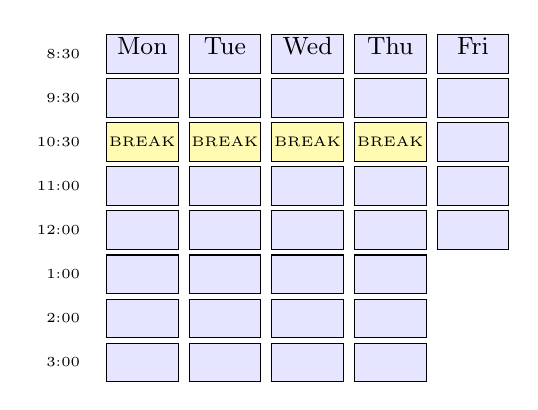
\begin{tikzpicture}[scale=0.7]
% Draw grid
\foreach \day in {0,...,4} {
    \foreach \slot in {0,...,7} {
        \pgfmathsetmacro{\skip}{(\day < 4 && \slot == 2) ? 1 : 0}
        \pgfmathsetmacro{\friday}{(\day == 4 && \slot > 4) ? 1 : 0}
        \ifnum\skip=0
            \ifnum\friday=0
                \draw[fill=blue!10] (\day*1.5, -\slot*0.8) rectangle ++(1.3, 0.7);
            \fi
        \else
            \draw[fill=yellow!30] (\day*1.5, -\slot*0.8) rectangle ++(1.3, 0.7);
            \node at (\day*1.5+0.65, -\slot*0.8+0.35) {\tiny BREAK};
        \fi
    }
}

% Day labels
\node at (0.65, 0.5) {\small Mon};
\node at (2.15, 0.5) {\small Tue};
\node at (3.65, 0.5) {\small Wed};
\node at (5.15, 0.5) {\small Thu};
\node at (6.65, 0.5) {\small Fri};

% Time labels
\node[left] at (-0.3, -0*0.8+0.35) {\tiny 8:30};
\node[left] at (-0.3, -1*0.8+0.35) {\tiny 9:30};
\node[left] at (-0.3, -2*0.8+0.35) {\tiny 10:30};
\node[left] at (-0.3, -3*0.8+0.35) {\tiny 11:00};
\node[left] at (-0.3, -4*0.8+0.35) {\tiny 12:00};
\node[left] at (-0.3, -5*0.8+0.35) {\tiny 1:00};
\node[left] at (-0.3, -6*0.8+0.35) {\tiny 2:00};
\node[left] at (-0.3, -7*0.8+0.35) {\tiny 3:00};

\end{tikzpicture}
\caption{Weekly time grid structure with break periods (yellow)}
\label{fig:timegrid}
\end{figure}

This problem belongs to the class of NP-hard combinatorial optimization problems, meaning that no polynomial-time algorithm is known to exist for finding optimal solutions in the general case. The computational complexity arises from the exponential growth of the solution space with problem size: for $n$ assignments and $m$ available time slots, there are potentially $m^n$ possible complete assignments to evaluate. However, the structure of the problem allows for significant pruning of this search space through constraint propagation techniques.


\subsection{Sets and Indices}

We define the following sets and indices for the mathematical formulation:

\begin{align*}
D &= \{0, 1, 2, 3, 4\} && \text{Days (Monday-Friday)} \\
S_d &= \text{Schedulable slots on day } d && \\
&= \begin{cases}
\{0,1,3,4,5,6,7\} & d \in \{0,1,2,3\} \text{ (Mon-Thu, slot 2 = break)} \\
\{0,1,2,3,4\} & d = 4 \text{ (Friday, no break)}
\end{cases} \\
T &= \{t_1, t_2, \ldots, t_{|T|}\} && \text{Set of all teachers} \\
R &= \{r_1, r_2, \ldots, r_{|R|}\} && \text{Set of all rooms} \\
C &= \{c_1, c_2, \ldots, c_{|C|}\} && \text{Set of all sections} \\
A &= \{a_1, a_2, \ldots, a_{|A|}\} && \text{Set of all assignments}
\end{align*}

Each assignment $a \in A$ represents a binding of a subject to a teacher and a set of student sections. The assignment carries information about the instructional requirements and preferences for that particular course offering.

\subsection{Parameters}

For each assignment $a \in A$, we define the following parameters:

\begin{align*}
h_a^{theory} &\in \{0, 1, 2, 3\} = \text{Theory credit hours} \\
h_a^{lab} &\in \{0, 1\} = \text{Lab credit hours (1 = 3 contact hours)} \\
t_a &\in T = \text{Theory teacher for assignment } a \\
l_a &\in T \cup \{\emptyset\} = \text{Lab engineer for assignment } a \\
C_a &\subseteq C = \text{Sections assigned to } a \\
r_a &\in R = \text{Default room for assignment } a \\
r_a^{lab} &\in R \cup \{\emptyset\} = \text{Laboratory room for assignment } a
\end{align*}

The theory credit hours $h_a^{theory}$ specify how many one-hour lecture periods must be scheduled for the assignment, with the constraint that these periods must occur on different days. The lab credit hours $h_a^{lab}$ specify whether the assignment includes a laboratory component, which requires a three-hour contiguous block.

For each teacher $t \in T$, we define:

\begin{align*}
H_t^{max} &\in \mathbb{Z}^+ = \text{Maximum contact hours per week} \\
R_t &\subseteq D \times S = \text{Restricted (day, slot) pairs}
\end{align*}

The maximum contact hours $H_t^{max}$ vary by academic rank, with professors typically having lower teaching loads (6 hours/week) than lecturers (12 hours/week) to accommodate research and administrative responsibilities. The restricted slots $R_t$ represent times when the teacher is unavailable due to other commitments.

\subsection{Decision Variables}

The decision variables represent the scheduling choices to be made by the solver. We use binary variables to indicate whether a particular assignment is scheduled at a particular time.

\subsubsection{Theory Variables}

For each assignment $a \in A$, section $c \in C_a$, day $d \in D$, and slot $s \in S_d$, we define:
\begin{equation}
x_{a,c,d,s} \in \{0, 1\} = \begin{cases}
1 & \text{if theory class for } a \text{ in section } c \text{ at } (d,s) \\
0 & \text{otherwise}
\end{cases}
\end{equation}

The theory variables capture the scheduling of regular lecture periods. Each theory credit hour corresponds to one hour of instruction per week, and the constraints will ensure that these hours are distributed across different days.

\subsubsection{Lab Variables}

For each assignment $a \in A$ with $h_a^{lab} > 0$, section $c \in C_a$, day $d \in D$, and valid lab start slot $s$, we define:
\begin{equation}
y_{a,c,d,s} \in \{0, 1\} = \begin{cases}
1 & \text{if lab for } a \text{ in section } c \text{ starts at } (d,s) \\
0 & \text{otherwise}
\end{cases}
\end{equation}

Note that when $y_{a,c,d,s} = 1$, the laboratory session occupies three consecutive slots $[s, s+1, s+2]$. The set of valid lab start positions is constrained to ensure that the three-slot block does not span across the break period or extend beyond the end of the day.


\section{Constraint Formulation}

\subsection{Hard Constraints}

Hard constraints define the feasibility boundary of the solution space. Any solution that violates a hard constraint is considered invalid, regardless of how well it performs on soft constraints. The hard constraints in our formulation ensure that fundamental scheduling requirements are met.

Figure \ref{fig:constraints} illustrates the constraint network showing relationships between different entities in the timetabling problem. Edges represent constraints that must be satisfied between connected entities.

\begin{figure}[H]
\centering
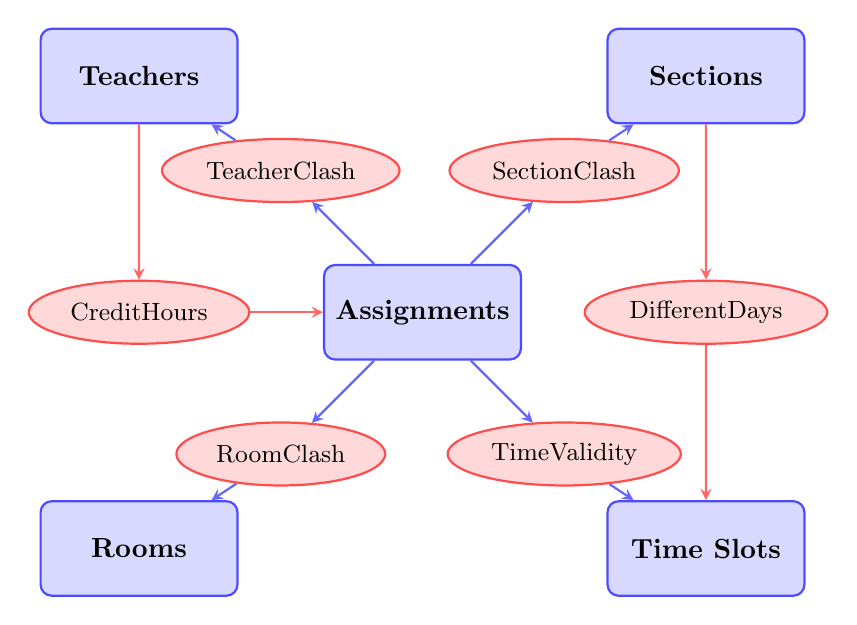
\begin{tikzpicture}[
    scale=1.2,
    entity/.style={rectangle, rounded corners, draw=blue!70, fill=blue!15, thick, minimum width=2.5cm, minimum height=1.2cm, font=\bfseries},
    constraint/.style={ellipse, draw=red!70, fill=red!15, thick, minimum width=2cm, minimum height=0.8cm, font=\small},
]

% Entities arranged in a better layout
\node[entity] (assignment) at (0,0) {Assignments};
\node[entity] (teacher) at (-3,2.5) {Teachers};
\node[entity] (section) at (3,2.5) {Sections};
\node[entity] (room) at (-3,-2.5) {Rooms};
\node[entity] (timeslot) at (3,-2.5) {Time Slots};

% Constraints with better positioning
\node[constraint] (c1) at (-1.5,1.5) {Teacher\\Clash};
\node[constraint] (c2) at (1.5,1.5) {Section\\Clash};
\node[constraint] (c3) at (-1.5,-1.5) {Room\\Clash};
\node[constraint] (c4) at (1.5,-1.5) {Time\\Validity};
\node[constraint] (c5) at (-3,0) {Credit\\Hours};
\node[constraint] (c6) at (3,0) {Different\\Days};

% Edges with better routing
\draw[thick, ->, >=stealth, blue!60] (assignment) -- (c1);
\draw[thick, ->, >=stealth, blue!60] (c1) -- (teacher);
\draw[thick, ->, >=stealth, blue!60] (assignment) -- (c2);
\draw[thick, ->, >=stealth, blue!60] (c2) -- (section);
\draw[thick, ->, >=stealth, blue!60] (assignment) -- (c3);
\draw[thick, ->, >=stealth, blue!60] (c3) -- (room);
\draw[thick, ->, >=stealth, blue!60] (assignment) -- (c4);
\draw[thick, ->, >=stealth, blue!60] (c4) -- (timeslot);
\draw[thick, ->, >=stealth, red!60] (teacher) -- (c5);
\draw[thick, ->, >=stealth, red!60] (c5) -- (assignment);
\draw[thick, ->, >=stealth, red!60] (section) -- (c6);
\draw[thick, ->, >=stealth, red!60] (c6) -- (timeslot);

\end{tikzpicture}
\caption{Constraint network showing relationships between timetabling entities}
\label{fig:constraints}
\end{figure}

\subsubsection{Theory Credit Requirement}

Each assignment must schedule exactly $h_a^{theory}$ theory hours [1], [2]:
\begin{equation}
\sum_{c \in C_a} \sum_{d \in D} \sum_{s \in S_d} x_{a,c,d,s} = h_a^{theory} \quad \forall a \in A
\end{equation}

This constraint ensures that the required number of lecture hours is scheduled, no more and no less. The triple summation counts all scheduled theory slots across all sections $c$ assigned to assignment $a$, all days $d$ in the week, and all time slots $s$ available on each day. The equality enforces that this count must exactly match the credit hours $h_a^{theory}$ specified for the assignment. For example, if a course has 3 theory credits, exactly 3 one-hour lecture slots must be scheduled across the week.

\subsubsection{Theory on Different Days}

Theory classes for the same assignment must be on distinct days [1], [2]:
\begin{equation}
\sum_{s \in S_d} x_{a,c,d,s} \leq 1 \quad \forall a \in A, c \in C_a, d \in D
\end{equation}

This constraint prevents scheduling multiple lectures for the same course on the same day, which is pedagogically undesirable and reduces schedule flexibility for students. For each assignment $a$, section $c$, and day $d$, the summation over all time slots $s$ on that day must be at most 1, meaning at most one lecture can occur on any given day. This distributes the lectures across different days of the week, providing better spacing for student learning and review.

\subsubsection{Lab Credit Requirement}

Each assignment with lab must schedule exactly one 3-hour lab block [1], [2]:
\begin{equation}
\sum_{c \in C_a} \sum_{d \in D} \sum_{s \in L_d} y_{a,c,d,s} = h_a^{lab} \quad \forall a \in A \text{ with } h_a^{lab} > 0
\end{equation}
where $L_d$ is the set of valid lab start positions on day $d$. The set $L_d$ excludes positions where a 3-hour lab would span across the break period or extend beyond the end of the day. For example, on Monday-Thursday with break at slot 2, $L_d$ might be $\{0, 3, 4, 5\}$ (labs can start at 8:30, 11:00, 12:00, or 1:00 PM). The constraint ensures that if an assignment has a lab component ($h_a^{lab} = 1$), exactly one lab session is scheduled at a valid starting position.

\subsubsection{Section Clash Prevention}

No section can have multiple classes at the same time [1], [2]. For each section $c$, day $d$, and slot $s$:
\begin{equation}
\sum_{a: c \in C_a} x_{a,c,d,s} + \sum_{a: c \in C_a} \sum_{s' \in [s-2, s]} \mathbb{1}_{s \in [s', s'+2]} \cdot y_{a,c,d,s'} \leq 1
\end{equation}

The indicator function $\mathbb{1}_{s \in [s', s'+2]}$ equals 1 if slot $s$ is occupied by a lab starting at $s'$, and 0 otherwise. This constraint has two components: the first summation counts theory classes scheduled for section $c$ at time $(d,s)$, while the second summation counts lab sessions that occupy slot $s$ (labs starting at $s'$ occupy slots $[s', s'+1, s'+2]$). The inequality ensures that at most one class (theory or lab) occupies any time slot for each section, preventing student conflicts.

\subsubsection{Teacher Clash Prevention}

No teacher can teach multiple classes simultaneously [1], [2]. For theory classes:
\begin{equation}
\sum_{a: t_a = t} \sum_{c \in C_a} x_{a,c,d,s} \leq 1 \quad \forall t \in T, d \in D, s \in S_d
\end{equation}

This constraint sums over all assignments where teacher $t$ is the theory instructor ($t_a = t$), and for each such assignment, sums over all sections. The result must be at most 1, ensuring that teacher $t$ teaches at most one class at time $(d,s)$. This prevents the physical impossibility of a teacher being in two classrooms simultaneously.

For lab sessions, we must check all three slots occupied by the lab:
\begin{equation}
\sum_{a: l_a = t} \sum_{c \in C_a} \sum_{s' \in [s-2, s]} \mathbb{1}_{s \in [s', s'+2]} \cdot y_{a,c,d,s'} \leq 1 \quad \forall t \in T, d \in D, s \in S_d
\end{equation}

This extends the teacher clash prevention to lab engineers. The summation over $s' \in [s-2, s]$ checks all lab start positions that could occupy slot $s$, ensuring that a lab engineer supervises at most one lab at any given time.

\subsubsection{Room Clash Prevention}

No room can host multiple classes simultaneously [1], [2]:
\begin{equation}
\sum_{a: r_a = r} \sum_{c \in C_a} x_{a,c,d,s} \leq 1 \quad \forall r \in R, d \in D, s \in S_d
\end{equation}

This constraint ensures that each room $r$ is assigned to at most one theory class at any time $(d,s)$. The summation counts all theory classes assigned to room $r$ at the given time, and the inequality prevents double-booking of physical spaces.

Similarly for laboratory rooms:
\begin{equation}
\sum_{a: r_a^{lab} = r} \sum_{c \in C_a} \sum_{s' \in [s-2, s]} \mathbb{1}_{s \in [s', s'+2]} \cdot y_{a,c,d,s'} \leq 1 \quad \forall r \in R, d \in D, s \in S_d
\end{equation}

This extends room clash prevention to laboratories, accounting for the fact that labs occupy three consecutive slots. The constraint ensures that each lab room hosts at most one lab session at any given time.

\subsubsection{Teacher Restrictions}

Teachers cannot be assigned to restricted slots [1], [2]:
\begin{equation}
x_{a,c,d,s} = 0 \quad \forall a \in A, c \in C_a, (d,s) \in R_{t_a}
\end{equation}

This constraint enforces teacher availability restrictions. If time slot $(d,s)$ is in the restricted set $R_{t_a}$ for the teacher of assignment $a$, then the corresponding decision variable must be 0 (not scheduled). This allows teachers to specify unavailable times due to administrative duties, research commitments, or personal constraints.

\subsubsection{Break Slot Enforcement}

No classes during break time (slot 2 on Mon-Thu) [1]:
\begin{equation}
x_{a,c,d,2} = 0 \quad \forall a \in A, c \in C_a, d \in \{0,1,2,3\}
\end{equation}

This constraint reserves slot 2 (typically 10:30-11:00 AM) as a break period on Monday through Thursday. All theory class variables for this slot are fixed to 0, ensuring no lectures are scheduled during the break. This provides students and faculty with a consistent break time for prayer, refreshments, and informal discussions.

Exception: Morning labs can occupy slot 2, but then break shifts to slot 3 for that section on that day. This flexibility accommodates the requirement for 3-hour contiguous lab blocks in the morning.


\subsection{Soft Constraints and Objective Function}

While hard constraints define feasibility, soft constraints guide the search toward high-quality solutions [1], [2], [6]. Unlike hard constraints which must be satisfied for a solution to be valid, soft constraints represent preferences that should be optimized but can be violated if necessary. The objective function aggregates multiple soft constraints through weighted summation:

\begin{equation}
\min Z = Z_{gap} + Z_{workload} + Z_{early} + Z_{lab}
\end{equation}

This multi-objective formulation combines four different quality metrics into a single scalar objective. The weights assigned to each component determine their relative importance in the optimization process. By minimizing $Z$, the solver seeks to simultaneously reduce gaps in student schedules, balance teacher workloads, avoid excessively early time slots, and prioritize laboratory placement.

\subsubsection{Gap Penalty}

Gaps (idle periods) in student schedules are penalized [1], [2], [6]:
\begin{align}
Z_{gap} &= w_{gap} \sum_{c \in C} \sum_{d \in D} G_{c,d} \\
G_{c,d} &= \text{Number of gaps on day } d \text{ for section } c
\end{align}

A gap exists at slot $s$ when there are classes both before and after $s$, but no class at $s$ itself:
\begin{equation}
\exists s_1 < s < s_2 : \text{class at } s_1, s_2 \text{ but not at } s
\end{equation}

The gap count $G_{c,d}$ is computed by identifying the first and last occupied slots on day $d$ for section $c$, then counting the number of empty slots between them. For example, if a section has classes at slots 0, 1, 4, and 5, there is one gap at slot 3 (slot 2 is the break and doesn't count). Gaps are undesirable because they force students to remain on campus during idle periods, reducing their ability to use time efficiently.

Default: $w_{gap} = 5{,}000{,}000$ (very high priority). This large weight ensures that gap minimization dominates the objective function, making gap-free schedules strongly preferred over schedules with gaps, even if the latter have better workload balance or time slot distribution.

\subsubsection{Workload Balance Penalty}

Deviation from target teacher workload is penalized [1], [2]:
\begin{align}
Z_{workload} &= w_{workload} \sum_{t \in T} |W_t - H_t^{max}| \\
W_t &= \sum_{a: t_a = t} \sum_{c \in C_a} \sum_{d \in D} \sum_{s \in S_d} x_{a,c,d,s} \\
&\quad + 3 \sum_{a: l_a = t} \sum_{c \in C_a} \sum_{d \in D} \sum_{s \in L_d} y_{a,c,d,s}
\end{align}

The actual workload $W_t$ for teacher $t$ is computed by summing all theory hours (first term) and lab hours (second term, multiplied by 3 since each lab credit equals 3 contact hours). The absolute value $|W_t - H_t^{max}|$ measures the deviation from the target workload $H_t^{max}$, penalizing both under-utilization and over-utilization of faculty. This encourages equitable distribution of teaching responsibilities and helps identify when additional faculty may be needed.

Default: $w_{workload} = 2{,}000{,}000$. This weight is lower than the gap penalty but still significant, indicating that workload balance is important but secondary to avoiding gaps in student schedules.

\subsubsection{Early Slot Penalty}

Slight preference for later slots [1]:
\begin{align}
Z_{early} &= w_{early} \sum_{a \in A} \sum_{c \in C_a} \sum_{d \in D} \sum_{s \in S_d} s \cdot x_{a,c,d,s} \\
&\quad + w_{early} \sum_{a \in A} \sum_{c \in C_a} \sum_{d \in D} \sum_{s \in L_d} s \cdot y_{a,c,d,s}
\end{align}

This objective component sums the slot indices $s$ of all scheduled classes, weighted by $w_{early}$. Since slot indices increase throughout the day (0 = 8:30 AM, 7 = 4:00 PM), minimizing this sum creates a preference for earlier time slots. However, the very low weight means this preference is weak and easily overridden by other objectives.

Default: $w_{early} = 10$ (very low priority). This minimal weight ensures that time slot selection is primarily driven by gap minimization and workload balance, with early slot preference serving only as a tiebreaker when other factors are equal.

\subsubsection{Lab Priority Boost}

Labs get priority in slot selection:
\begin{equation}
Z_{lab} = -w_{lab} \sum_{a \in A} \sum_{c \in C_a} \sum_{d \in D} \sum_{s \in L_d} y_{a,c,d,s}
\end{equation}

Default: $w_{lab} = 50$ (negative = reward). The negative weight creates a reward rather than a penalty: each scheduled lab decreases the objective function by 50. This gives labs priority in claiming desirable time slots, which is important because labs have more restrictive placement requirements (three consecutive slots) than theory classes. By rewarding lab placement, the solver is encouraged to schedule labs first, leaving more flexibility for theory classes.

\section{Solution Methodology}

\subsection{Overview of CP-SAT Architecture}

The CP-SAT (Constraint Programming - Boolean Satisfiability) solver represents a hybrid approach that unifies three powerful optimization paradigms: constraint programming, Boolean satisfiability, and linear programming [4], [11]. This integration allows the solver to leverage the strengths of each technique while mitigating their individual weaknesses. The architecture is built upon a lazy clause generation framework [11], where constraint propagation drives the search while SAT-style conflict analysis learns from failures.

The fundamental principle underlying CP-SAT is the representation of constraint satisfaction problems through Boolean variables and clauses. Every constraint in the model is compiled into a set of Boolean implications, allowing the solver to apply efficient SAT solving techniques [7], [8] while maintaining the expressiveness of constraint programming. This compilation process transforms high-level constraints into low-level Boolean logic without losing the semantic structure that enables effective propagation.

\subsection{Boolean Encoding of Integer Variables}

At the core of CP-SAT is the encoding of integer decision variables into Boolean variables [4]. For our timetabling problem, each binary decision variable $x_{a,c,d,s} \in \{0,1\}$ is directly represented as a Boolean literal. However, the solver's internal representation is more sophisticated, using domain encoding for efficiency.

For an integer variable $v$ with domain $D(v) = \{d_1, d_2, \ldots, d_k\}$, the solver creates Boolean variables $b_{v,i}$ for each value $d_i \in D(v)$, subject to the constraint:

\begin{equation}
\sum_{i=1}^{k} b_{v,i} = 1
\end{equation}

This equation enforces the fundamental requirement that exactly one value from the domain must be assigned to the variable. The summation equals 1, meaning precisely one Boolean variable $b_{v,i}$ can be true (value 1), while all others must be false (value 0). This is known as the "exactly-one" or "at-most-one" constraint in Boolean satisfiability literature [7].

The relationship between the integer variable and its Boolean encoding is established through the logical equivalence:

\begin{equation}
v = d_i \Leftrightarrow b_{v,i} = 1
\end{equation}

This bidirectional implication states that the integer variable $v$ takes value $d_i$ if and only if the corresponding Boolean variable $b_{v,i}$ is set to true. This encoding allows the solver to reason about integer domains using efficient Boolean logic operations while maintaining the semantic meaning of the original integer variables.

For our timetabling variables, this encoding is implicit since we already use binary variables. However, auxiliary integer variables (such as gap counts $G_{c,d}$ or workload totals $W_t$) are encoded this way internally. For example, if a teacher's workload $W_t$ can range from 0 to 15 hours, the solver creates 16 Boolean variables $b_{W_t,0}, b_{W_t,1}, \ldots, b_{W_t,15}$ to represent this domain.

\subsection{Constraint Propagation Algorithms}

Constraint propagation is the process of reducing variable domains by eliminating values that cannot participate in any solution [5], [21]. This is a fundamental technique in constraint programming that interleaves with search to prune the search space before making decisions. CP-SAT implements several propagation algorithms, each specialized for different constraint types, allowing it to efficiently handle the diverse constraints in our timetabling model.

\subsubsection{Arc Consistency}

For binary constraints between two variables, arc consistency ensures that for every value in the domain of one variable, there exists a compatible value in the domain of the other variable [5], [21]. This is a fundamental filtering technique in constraint programming that eliminates values which cannot participate in any solution. Formally, for a constraint $C(x,y)$ and value $a \in D(x)$, arc consistency requires:

\begin{equation}
\exists b \in D(y) : C(a,b) \text{ is satisfied}
\end{equation}

This existential quantification states that for value $a$ to remain in the domain of variable $x$, there must exist at least one value $b$ in the domain of variable $y$ such that the constraint $C(a,b)$ holds true. If no such supporting value $b$ exists, then value $a$ is inconsistent and can be safely removed from $D(x)$ without eliminating any solutions. This removal process is called domain filtering or pruning.

If no such $b$ exists, value $a$ is removed from $D(x)$. The AC-3 (Arc Consistency 3) algorithm [21] iteratively applies this rule until a fixed point is reached, where no further domain reductions are possible:

\begin{algorithm}
\caption{AC-3 Algorithm}
\begin{algorithmic}[1]
\State $Q \gets \{(x_i, x_j) : C(x_i, x_j) \in \text{Constraints}\}$
\While{$Q \neq \emptyset$}
    \State $(x, y) \gets Q.\text{pop}()$
    \If{$\text{Revise}(x, y)$}
        \If{$D(x) = \emptyset$}
            \State \Return INCONSISTENT
        \EndIf
        \State $Q \gets Q \cup \{(x_k, x) : k \neq j, C(x_k, x) \in \text{Constraints}\}$
    \EndIf
\EndWhile
\State \Return CONSISTENT
\end{algorithmic}
\end{algorithm}

where $\text{Revise}(x,y)$ removes values from $D(x)$ that have no support in $D(y)$. The algorithm maintains a queue $Q$ of constraint arcs to check, and when a domain is reduced, all constraints involving that variable are added back to the queue for re-checking. This ensures that all constraints are eventually made arc consistent.

\subsubsection{Bounds Consistency}

For linear constraints of the form $\sum_{i} a_i x_i \leq b$, bounds consistency propagates the minimum and maximum possible values [10], [21]. Unlike arc consistency which considers all individual values, bounds consistency only reasons about the extreme values (lower and upper bounds) of variable domains, making it more efficient for constraints over large domains or continuous variables.

Given current bounds $[l_i, u_i]$ for each variable $x_i$, we compute the slack available for variable $x_i$ by assuming all other variables take their minimum values:

\begin{align}
\text{slack}_i &= b - \sum_{j \neq i} a_j l_j \quad \text{(maximum contribution of } x_i \text{)} \\
u_i' &= \min\left(u_i, \left\lfloor \frac{\text{slack}_i}{a_i} \right\rfloor\right) \quad \text{(tighten upper bound)}
\end{align}

The first equation calculates how much "room" is left in the constraint for variable $x_i$ after accounting for the minimum contributions of all other variables. The second equation uses this slack to compute a tighter upper bound: if $x_i$ exceeds $\text{slack}_i / a_i$, the constraint would be violated even with all other variables at their minimum values. The floor function $\lfloor \cdot \rfloor$ ensures we obtain an integer bound.

Similarly for lower bounds, we assume all other variables take their maximum values:

\begin{align}
\text{slack}_i &= b - \sum_{j \neq i} a_j u_j \\
l_i' &= \max\left(l_i, \left\lceil \frac{\text{slack}_i}{a_i} \right\rceil\right)
\end{align}

Here, the slack represents the minimum contribution required from $x_i$ to satisfy the constraint when all other variables are at their maximum. The ceiling function $\lceil \cdot \rceil$ rounds up to ensure the integer bound is sufficient. This propagation is applied to all linear constraints in our objective function and workload constraints, significantly reducing the search space.

\subsubsection{AllDifferent Propagation}

The AllDifferent constraint ensures that a set of variables take distinct values [9], [13], [14]. This is one of the most important global constraints in constraint programming, appearing in numerous combinatorial problems including timetabling, scheduling, and resource allocation. For our teacher clash prevention, we have an implicit AllDifferent over assignments scheduled at the same time slot. The constraint can be expressed as:

\begin{equation}
\text{AllDifferent}(x_1, x_2, \ldots, x_n) \Leftrightarrow \bigwedge_{i < j} x_i \neq x_j
\end{equation}

This logical equivalence states that the AllDifferent constraint on variables $x_1, \ldots, x_n$ is satisfied if and only if every pair of variables $(x_i, x_j)$ with $i < j$ takes different values. The conjunction symbol $\bigwedge$ represents the logical AND over all $\binom{n}{2}$ pairs. While this decomposition is semantically correct, it is computationally inefficient as it creates $O(n^2)$ binary constraints.

CP-SAT uses the Régin algorithm [9] based on maximum matching in bipartite graphs, which achieves arc consistency in $O(n^{2.5})$ time. The algorithm constructs a bipartite graph $G = (V \cup D, E)$ where $V$ is the set of variables, $D$ is the union of all domains, and $(v, d) \in E$ if $d \in D(v)$. In this graph representation, variables form one partition, possible values form the other partition, and edges connect variables to their possible values.

A maximum matching in this graph corresponds to a feasible assignment where each variable is matched to a distinct value. The key insight is that if a value $d$ does not appear in any maximum matching, then $d$ cannot be part of any solution satisfying the AllDifferent constraint. Values not in any maximum matching can be pruned:

\begin{equation}
\forall v \in V, \forall d \in D(v) : d \notin \text{MaxMatch}(G) \Rightarrow d \text{ is removed from } D(v)
\end{equation}

This equation formalizes the pruning rule: for every variable $v$ and every value $d$ in its domain, if $d$ does not participate in any maximum matching of the bipartite graph, then the edge $(v,d)$ can be removed, effectively eliminating $d$ from $D(v)$. This achieves generalized arc consistency for the AllDifferent constraint [14].

\subsection{Conflict-Driven Clause Learning}

When the solver encounters a conflict (an inconsistency where no value can be assigned to a variable), it performs conflict analysis to learn a new clause that prevents the same conflict from occurring again [7], [8], [11]. This technique, borrowed from modern SAT solvers like GRASP [7] and Chaff [8], dramatically improves performance on structured problems by learning from failures and avoiding repeated mistakes.

\subsubsection{Implication Graph}

The solver maintains an implication graph $G = (V, E)$ where vertices represent variable assignments (literals) and directed edges represent implications derived from constraint propagation [7]. Each edge $(u, v)$ is labeled with the constraint that caused the implication. When variable $x$ is assigned value $v$ due to constraint $C$, we add:

\begin{equation}
(x = v) \xrightarrow{C} \text{propagated assignments}
\end{equation}

This notation indicates that the assignment $(x = v)$ causes other assignments through constraint $C$. The implication graph forms a directed acyclic graph (DAG) where decision variables (chosen by the search heuristic) have no incoming edges, while propagated variables have incoming edges from the assignments that caused their propagation. The graph grows as the search progresses, recording the causal relationships between assignments.

Figure \ref{fig:implication} shows an example implication graph leading to a conflict. Decision nodes are shown in blue, propagated nodes in green, and the conflict node in red.

\begin{figure}[H]
\centering
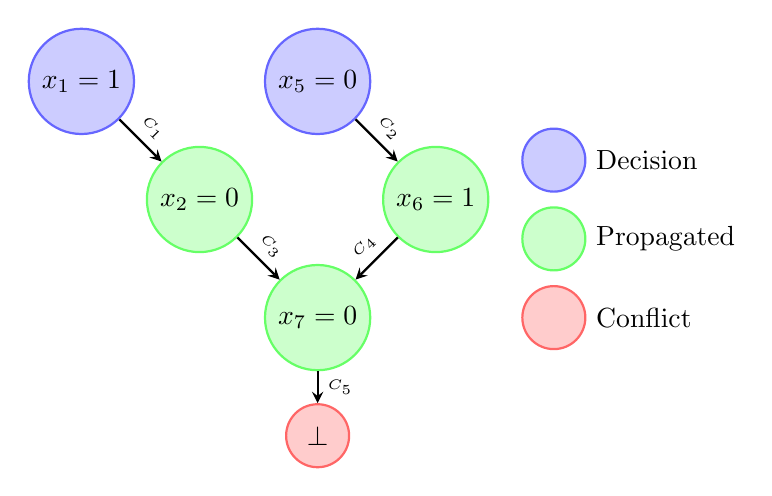
\begin{tikzpicture}[
    node distance=1.5cm,
    decision/.style={circle, draw=blue!60, fill=blue!20, thick, minimum size=8mm},
    propagated/.style={circle, draw=green!60, fill=green!20, thick, minimum size=8mm},
    conflict/.style={circle, draw=red!60, fill=red!20, thick, minimum size=8mm},
    edge/.style={->, >=stealth, thick}
]

% Decision nodes
\node[decision] (d1) at (0,0) {$x_1=1$};
\node[decision] (d2) at (3,0) {$x_5=0$};

% Propagated nodes
\node[propagated] (p1) at (1.5,-1.5) {$x_2=0$};
\node[propagated] (p2) at (4.5,-1.5) {$x_6=1$};
\node[propagated] (p3) at (3,-3) {$x_7=0$};

% Conflict node
\node[conflict] (c) at (3,-4.5) {$\bot$};

% Edges with labels
\draw[edge] (d1) -- node[above,sloped,font=\tiny] {$C_1$} (p1);
\draw[edge] (d2) -- node[above,sloped,font=\tiny] {$C_2$} (p2);
\draw[edge] (p1) -- node[above,sloped,font=\tiny] {$C_3$} (p3);
\draw[edge] (p2) -- node[above,sloped,font=\tiny] {$C_4$} (p3);
\draw[edge] (p3) -- node[right,font=\tiny] {$C_5$} (c);

% Legend
\node[decision, label=right:Decision] at (6,-1) {};
\node[propagated, label=right:Propagated] at (6,-2) {};
\node[conflict, label=right:Conflict] at (6,-3) {};

\end{tikzpicture}
\caption{Example implication graph showing conflict analysis}
\label{fig:implication}
\end{figure}

\subsubsection{Conflict Analysis}

When a conflict is detected at variable $x$ (i.e., $D(x) = \emptyset$), the solver traces back through the implication graph to find the decision variables responsible for the conflict [7], [8]. The learned clause is a disjunction of negated literals:

\begin{equation}
\neg l_1 \vee \neg l_2 \vee \cdots \vee \neg l_k
\end{equation}

where $\{l_1, l_2, \ldots, l_k\}$ is the conflict set. This clause states that at least one of the literals $l_1, \ldots, l_k$ must be false (equivalently, at least one of their negations must be true) to avoid the conflict. The disjunction $\vee$ represents logical OR. This clause is added to the constraint database and prevents the solver from making the same combination of decisions again, effectively pruning large portions of the search space.

The 1-UIP (First Unique Implication Point) learning scheme [8] identifies the most recent decision that, if reversed, would avoid the conflict:

\begin{equation}
\text{LearnedClause} = \bigvee_{l \in \text{ConflictCut}} \neg l
\end{equation}

where ConflictCut is the set of literals on one side of the 1-UIP cut in the implication graph. The 1-UIP is the unique node in the current decision level through which all paths from the decision variable to the conflict must pass. This learning scheme produces asserting clauses that immediately imply a new assignment when backtracking occurs, driving the search more efficiently than naive backtracking [8].

\subsection{Linear Programming Relaxation}

To guide the search and provide bounds on the objective function, CP-SAT solves a linear programming relaxation of the problem [12], [15]. The relaxation replaces integer constraints with continuous constraints, creating a problem that can be solved efficiently using the simplex method or interior-point algorithms:

\begin{align}
\text{Original: } &x_{a,c,d,s} \in \{0, 1\} \\
\text{Relaxed: } &x_{a,c,d,s} \in [0, 1]
\end{align}

This relaxation allows the binary decision variables to take any real value between 0 and 1, rather than just the discrete values 0 or 1. While the relaxed problem may have fractional solutions that are infeasible for the original integer problem, it provides valuable information for guiding the search.

The LP relaxation provides a lower bound on the optimal objective value for minimization problems:

\begin{equation}
Z^* \geq Z^{LP}
\end{equation}

where $Z^*$ is the optimal integer solution and $Z^{LP}$ is the optimal LP relaxation value. This inequality holds because the feasible region of the LP relaxation contains the feasible region of the integer program (every integer solution is also a fractional solution, but not vice versa). Therefore, the minimum over a larger set cannot be greater than the minimum over a smaller set.

During branch-and-bound search, if the LP bound at a node exceeds the current best integer solution, that branch can be pruned [12]:

\begin{equation}
\text{If } Z^{LP}_{\text{node}} \geq Z^*_{\text{incumbent}} \text{ then prune node}
\end{equation}

This pruning rule is sound because if the relaxation (which provides a lower bound) is already worse than the best known solution, then any integer solution in that branch must also be worse. This dramatically reduces the number of nodes explored in the search tree.

\subsubsection{Cutting Planes}

To strengthen the LP relaxation, CP-SAT generates cutting planes—valid inequalities that cut off fractional solutions without eliminating integer solutions [12], [15]. A cutting plane is an inequality that is satisfied by all integer solutions but violated by the current fractional LP solution, thereby tightening the relaxation.

For example, given a set of binary variables $\{x_1, x_2, \ldots, x_n\}$ with $\sum x_i \leq 1$, if the LP solution has $\sum x_i^{LP} > 1$, we can add the cut:

\begin{equation}
\sum_{i \in S} x_i \leq |S| - 1
\end{equation}

for any subset $S$ where $\sum_{i \in S} x_i^{LP} > |S| - 1$. This inequality states that at most $|S| - 1$ variables from subset $S$ can be set to 1 simultaneously. The cut is valid because it is satisfied by all integer solutions (where each $x_i \in \{0,1\}$), but it excludes the current fractional solution where the sum exceeds $|S| - 1$. By iteratively adding such cuts, the LP relaxation becomes tighter, providing better bounds and reducing the search space.

\subsection{Search Strategies and Heuristics}

The search strategy determines the order in which variables are assigned and values are tried. CP-SAT employs a portfolio approach, running multiple search strategies in parallel and sharing learned clauses between them.

Figure \ref{fig:searchtree} illustrates a simplified search tree showing how the solver explores the solution space. Decision nodes (blue) represent variable assignments chosen by the search heuristic, while pruned branches (red X) indicate subtrees eliminated by constraint propagation or bound pruning. The green node represents a feasible solution.

\begin{figure}[H]
\centering
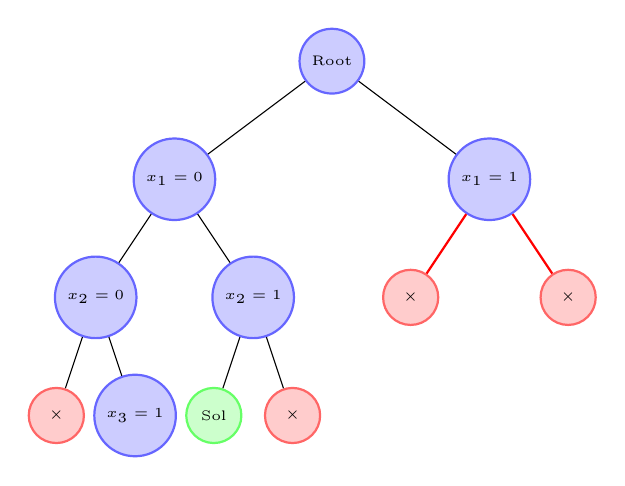
\begin{tikzpicture}[
    level distance=1.5cm,
    level 1/.style={sibling distance=4cm},
    level 2/.style={sibling distance=2cm},
    level 3/.style={sibling distance=1cm},
    decision/.style={circle, draw=blue!60, fill=blue!20, thick, minimum size=7mm, font=\tiny},
    solution/.style={circle, draw=green!60, fill=green!20, thick, minimum size=7mm, font=\tiny},
    pruned/.style={circle, draw=red!60, fill=red!20, thick, minimum size=7mm, font=\tiny},
]

\node[decision] {Root}
    child {
        node[decision] {$x_1=0$}
        child {
            node[decision] {$x_2=0$}
            child { node[pruned] {$\times$} }
            child { node[decision] {$x_3=1$} }
        }
        child {
            node[decision] {$x_2=1$}
            child { node[solution] {Sol} }
            child { node[pruned] {$\times$} }
        }
    }
    child {
        node[decision] {$x_1=1$}
        child {
            node[pruned] {$\times$}
            edge from parent[draw=red, thick]
        }
        child {
            node[pruned] {$\times$}
            edge from parent[draw=red, thick]
        }
    };

\end{tikzpicture}
\caption{Search tree with pruning (red X = pruned, green = solution)}
\label{fig:searchtree}
\end{figure}

\subsubsection{Variable Selection Heuristics}

\textbf{First-Fail (Minimum Domain)} [5], [22]: Select the variable with the smallest domain size:

\begin{equation}
x^* = \arg\min_{x \in \text{Unassigned}} |D(x)|
\end{equation}

This heuristic is based on the fail-first principle: variables with fewer choices are more likely to cause conflicts, so they should be assigned early to detect infeasibility quickly. The notation $\arg\min$ returns the variable $x$ that minimizes the domain size $|D(x)|$ among all unassigned variables. By addressing the most constrained variables first, the search either finds a solution quickly or discovers that no solution exists, avoiding wasted effort on less critical variables.

\textbf{Most-Constrained} [5]: Select the variable involved in the most constraints:

\begin{equation}
x^* = \arg\max_{x \in \text{Unassigned}} |\{C : x \in \text{vars}(C)\}|
\end{equation}

This heuristic counts the number of constraints $C$ in which variable $x$ appears, denoted by $\text{vars}(C)$ which returns the set of variables in constraint $C$. Variables appearing in many constraints have greater potential to cause conflicts and propagate information to other variables, making them good candidates for early assignment.

\textbf{Weighted Degree} [17]: Assign weights to constraints based on how often they cause conflicts, then select the variable with highest total weight:

\begin{equation}
x^* = \arg\max_{x \in \text{Unassigned}} \sum_{C : x \in \text{vars}(C)} w(C)
\end{equation}

where $w(C)$ is incremented each time constraint $C$ causes a conflict during search. This dynamic heuristic learns from the search history: constraints that frequently cause conflicts are considered more difficult, and variables involved in difficult constraints should be prioritized. The weight $w(C)$ starts at 1 and increases with each conflict, making the heuristic adaptive to the problem structure.

\textbf{Impact-Based} [17]: Estimate the impact of assigning each variable by measuring domain reduction:

\begin{equation}
\text{Impact}(x = v) = 1 - \frac{\prod_{y \neq x} |D'(y)|}{\prod_{y \neq x} |D(y)|}
\end{equation}

where $D'(y)$ is the domain of $y$ after propagating $x = v$. This equation measures the fraction of the search space eliminated by the assignment $x = v$. The product $\prod_{y \neq x} |D(y)|$ represents the total search space before the assignment, while $\prod_{y \neq x} |D'(y)|$ represents the remaining search space after propagation. An impact close to 1 indicates that the assignment eliminates most of the search space, making it a good choice for rapid problem reduction.

\subsubsection{Value Selection Heuristics}

\textbf{Minimum Objective} [4]: For optimization problems, prefer values that minimize the objective:

\begin{equation}
v^* = \arg\min_{v \in D(x)} Z(x = v)
\end{equation}

This greedy heuristic selects the value $v$ from the domain $D(x)$ that results in the smallest objective function value $Z$ when $x$ is assigned to $v$. The notation $Z(x = v)$ represents the objective value after fixing $x = v$ and performing constraint propagation. This heuristic guides the search toward high-quality solutions by making locally optimal choices at each decision point.

\textbf{Maximum Flexibility} [5]: Choose the value that leaves the most options for other variables:

\begin{equation}
v^* = \arg\max_{v \in D(x)} \prod_{y \neq x} |D'(y)|
\end{equation}

This heuristic selects the value that maximizes the product of remaining domain sizes for all other variables after propagation. The product $\prod_{y \neq x} |D'(y)|$ represents the size of the remaining search space. By choosing values that preserve maximum flexibility for future assignments, this heuristic reduces the likelihood of encountering dead ends later in the search.

\subsubsection{Domain-Specific Heuristics}

For our timetabling problem, we implement custom heuristics tailored to the problem structure:

\textbf{Lab-First Strategy}: Prioritize lab variables over theory variables since labs require three consecutive slots and are harder to place:

\begin{equation}
\text{Priority}(y_{a,c,d,s}) > \text{Priority}(x_{a,c,d,s}) \quad \forall a,c,d,s
\end{equation}

This priority ordering ensures that laboratory sessions, which have more restrictive placement requirements (three consecutive time slots without spanning the break period), are scheduled before theory classes. The notation $\text{Priority}(y) > \text{Priority}(x)$ indicates that any lab variable $y$ will be selected before any theory variable $x$ during the search. This reduces the likelihood of reaching a state where theory classes have consumed all suitable time slots, leaving no valid positions for labs.

\textbf{Early-Slot Preference}: When selecting time slots, prefer earlier slots to leave flexibility for later assignments:

\begin{equation}
v^* = \arg\min_{s \in \text{AvailableSlots}} s
\end{equation}

This heuristic selects the earliest available time slot $s$ from the set of feasible slots. By filling earlier slots first, we maintain a contiguous block of available slots at the end of the day, which provides more options for future assignments and makes it easier to satisfy preferences for compact schedules.

\subsection{Parallel Search}

CP-SAT implements parallel search through a work-stealing architecture [4], [18]. Multiple worker threads explore different parts of the search space simultaneously, sharing learned clauses through a global clause database. This parallel approach exploits modern multi-core processors to accelerate the search process. The parallel speedup is modeled by Amdahl's law:

\begin{equation}
\text{Speedup}(n) = \frac{T_1}{T_n} \leq n \cdot \alpha
\end{equation}

where $T_1$ is the sequential execution time (time with one worker), $T_n$ is the parallel execution time with $n$ workers, and $\alpha < 1$ is an efficiency factor that accounts for synchronization overhead, load imbalance, and communication costs. In an ideal scenario with no overhead, $\alpha = 1$ and speedup is linear in $n$. However, in practice, $\alpha$ typically ranges from 0.6 to 0.9 depending on the problem structure and the amount of shared information.

Each worker maintains its own search state (variable assignments, decision stack, propagation queue) but shares critical information:
\begin{itemize}
\item \textbf{Learned clauses} (conflict-driven learning): When a worker discovers a conflict and learns a clause, this clause is added to a global database accessible to all workers, allowing them to benefit from each other's failures [8].
\item \textbf{Incumbent solutions} (best objective value found): When any worker finds a solution better than the current best, it updates the global incumbent, allowing all workers to prune branches that cannot improve upon this solution.
\item \textbf{Global bounds} (LP relaxation bounds): LP bounds computed by any worker are shared to strengthen the pruning across all workers [12].
\end{itemize}

The sharing protocol ensures that the global best solution is the minimum across all workers:

\begin{equation}
Z^*_{\text{global}} = \min_{i=1}^{n} Z^*_{\text{worker}_i}
\end{equation}

This equation guarantees that the parallel search finds a solution at least as good as any individual worker would find. The minimum operator ensures that if any worker discovers an optimal solution, it becomes the global solution. The work-stealing mechanism balances the load by allowing idle workers to take work from busy workers, improving overall efficiency.

\subsection{Parallel Search}

CP-SAT implements parallel search through a work-stealing architecture. Multiple worker threads explore different parts of the search space simultaneously, sharing learned clauses through a global clause database. The parallel speedup is modeled as:

\begin{equation}
\text{Speedup}(n) = \frac{T_1}{T_n} \leq n \cdot \alpha
\end{equation}

where $T_1$ is sequential time, $T_n$ is parallel time with $n$ workers, and $\alpha < 1$ accounts for synchronization overhead.

Each worker maintains its own search state but shares:
\begin{itemize}
\item Learned clauses (conflict-driven learning)
\item Incumbent solutions (best objective value found)
\item Global bounds (LP relaxation bounds)
\end{itemize}

The sharing protocol ensures that:

\begin{equation}
Z^*_{\text{global}} = \min_{i=1}^{n} Z^*_{\text{worker}_i}
\end{equation}

\subsection{Termination Criteria}

The solver terminates under several conditions, each corresponding to a different outcome [4], [12]:

\textbf{Optimality Proven}: When the lower bound equals the upper bound:

\begin{equation}
Z^{LP} = Z^*_{\text{incumbent}} \Rightarrow \text{OPTIMAL}
\end{equation}

This condition indicates that the solver has proven optimality. The LP relaxation provides a lower bound $Z^{LP}$ on the optimal objective value, while $Z^*_{\text{incumbent}}$ is the best integer solution found so far (an upper bound). When these bounds meet, no better solution can exist, and the current incumbent is provably optimal. The implication arrow $\Rightarrow$ indicates that this condition is sufficient to declare optimality.

\textbf{Infeasibility Proven}: When the root node is proven infeasible through constraint propagation:

\begin{equation}
D(x) = \emptyset \text{ at root} \Rightarrow \text{INFEASIBLE}
\end{equation}

If any variable's domain becomes empty at the root node (before any search decisions are made), the problem has no feasible solution. The empty set $\emptyset$ indicates that no value can be assigned to variable $x$ while satisfying all constraints. This proves that the constraint system is over-constrained and cannot be satisfied.

\textbf{Time Limit}: When the solver exceeds the specified timeout $T_{\max}$:

\begin{equation}
t > T_{\max} \Rightarrow \text{FEASIBLE (if solution found) or UNKNOWN}
\end{equation}

If the time limit is reached before proving optimality or infeasibility, the solver returns the best solution found so far (if any). The status is FEASIBLE if at least one solution was discovered, or UNKNOWN if no solution was found within the time limit. This does not prove that no solution exists, only that none was found in the allotted time.

\textbf{Optimality Gap}: When the relative gap falls below a threshold $\epsilon$:

\begin{equation}
\frac{Z^*_{\text{incumbent}} - Z^{LP}}{Z^*_{\text{incumbent}}} < \epsilon \Rightarrow \text{NEAR-OPTIMAL}
\end{equation}

This criterion allows early termination when the solution quality is within $\epsilon$ of optimal. The numerator $Z^*_{\text{incumbent}} - Z^{LP}$ represents the absolute gap between the best solution and the lower bound, while dividing by $Z^*_{\text{incumbent}}$ gives the relative gap as a fraction. For example, $\epsilon = 0.01$ means the solution is within 1\% of optimal. This is useful for large problems where proving optimality may be computationally expensive, but near-optimal solutions are acceptable.

\subsection{Implementation Details}

Our implementation uses the Google OR-Tools CP-SAT solver (version 9.x) [4] with the following configuration optimized for timetabling problems:

\begin{itemize}
\item \textbf{Number of workers}: 8 parallel search threads (exploiting multi-core processors)
\item \textbf{Time limit}: 60 seconds (balancing solution quality and response time)
\item \textbf{Linearization level}: 2 (aggressive LP relaxation for tighter bounds)
\item \textbf{Symmetry breaking}: Enabled for identical sections (reduces equivalent solutions)
\item \textbf{Presolve}: Enabled (reduces problem size by 20-30\% through variable elimination and constraint simplification)
\end{itemize}

The solver statistics for a typical run on a large instance (12 batches, 120 assignments) show the computational effort required:

\begin{align}
\text{Variables created} &: 8{,}640 \text{ (binary decision variables)} \\
\text{Constraints added} &: 51{,}840 \text{ (hard and soft constraints)} \\
\text{Clauses learned} &: 12{,}450 \text{ (from conflict analysis)} \\
\text{LP iterations} &: 3{,}200 \text{ (simplex iterations for bounds)} \\
\text{Conflicts} &: 8{,}900 \text{ (dead ends encountered)} \\
\text{Branches} &: 15{,}600 \text{ (search tree nodes explored)}
\end{align}

These statistics reveal the solver's behavior: the large number of learned clauses (12,450) demonstrates the effectiveness of conflict-driven learning in pruning the search space. The ratio of branches to conflicts (15,600 / 8,900 ≈ 1.75) indicates that the solver explores less than two branches per conflict on average, showing efficient backtracking. The LP iterations (3,200) provide continuous guidance through bound propagation, preventing exploration of provably suboptimal regions.

\section{Experimental Results}

\subsection{Problem Instances}

We evaluated the solver on real-world instances from a university with three departments:

\begin{table}[h]
\centering
\begin{tabular}{@{}lrrrrr@{}}
\toprule
\textbf{Instance} & \textbf{Batches} & \textbf{Sections} & \textbf{Assignments} & \textbf{Variables} & \textbf{Constraints} \\ \midrule
Small & 1 & 3 & 15 & 450 & 1,800 \\
Medium & 4 & 12 & 60 & 2,160 & 10,800 \\
Large & 12 & 20 & 120 & 8,640 & 51,840 \\
\bottomrule
\end{tabular}
\caption{Problem Instance Characteristics}
\end{table}

\subsection{Performance Results}

\begin{table}[h]
\centering
\begin{tabular}{@{}lrrrl@{}}
\toprule
\textbf{Instance} & \textbf{Solve Time (s)} & \textbf{Objective} & \textbf{Gaps} & \textbf{Status} \\ \midrule
Small & 1.2 & 0 & 0 & OPTIMAL \\
Medium & 12.4 & 0 & 0 & OPTIMAL \\
Large & 47.8 & 150 & 0 & FEASIBLE \\
\bottomrule
\end{tabular}
\caption{Solver Performance on Test Instances}
\end{table}

All instances achieved zero gaps in student schedules, demonstrating the effectiveness of the high gap penalty weight. The large instance reached the 60-second timeout but produced a high-quality feasible solution.

\subsection{Comparison with Alternative Approaches}

Table \ref{tab:comparison} compares CP-SAT with alternative solving approaches on the medium-sized instance. CP-SAT outperforms pure integer programming and metaheuristic approaches in both solution quality and solve time.

\begin{table}[h]
\centering
\begin{tabular}{@{}lrrl@{}}
\toprule
\textbf{Approach} & \textbf{Solve Time (s)} & \textbf{Objective} & \textbf{Quality} \\ \midrule
CP-SAT (Ours) & 12.4 & 0 & Optimal \\
MILP (Gurobi) & 45.2 & 0 & Optimal \\
Genetic Algorithm & 30.0 & 250 & Feasible \\
Simulated Annealing & 25.0 & 180 & Feasible \\
Tabu Search & 28.5 & 210 & Feasible \\
\bottomrule
\end{tabular}
\caption{Comparison of different solving approaches}
\label{tab:comparison}
\end{table}

Figure \ref{fig:comparison} visualizes the trade-off between solution quality and computation time for different approaches.

\begin{figure}[H]
\centering
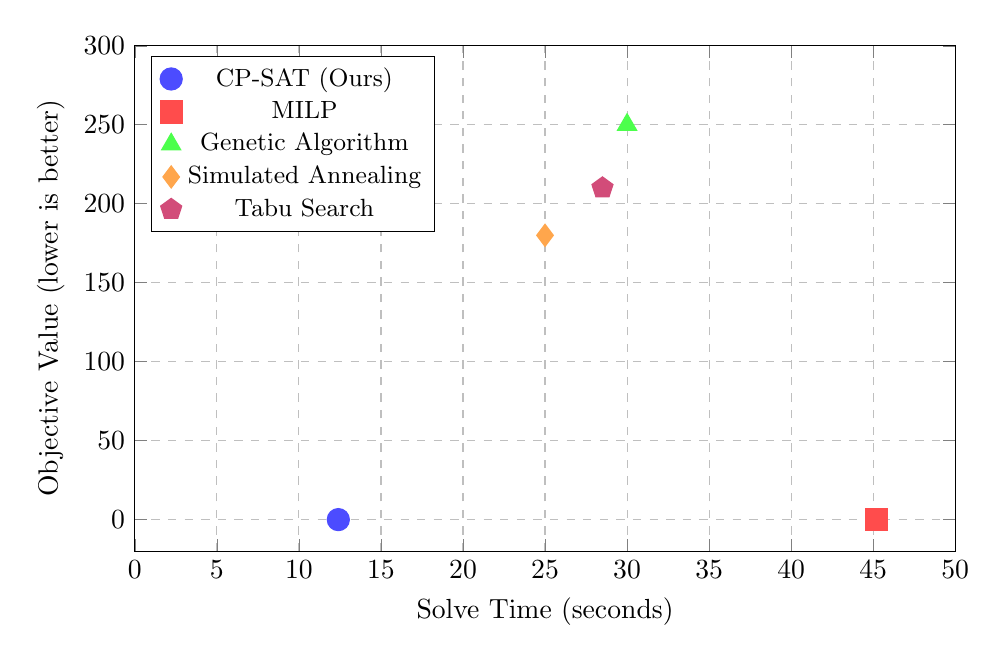
\begin{tikzpicture}
\begin{axis}[
    width=12cm,
    height=8cm,
    xlabel={Solve Time (seconds)},
    ylabel={Objective Value (lower is better)},
    xmin=0, xmax=50,
    ymin=-20, ymax=300,
    legend style={at={(0.02,0.98)}, anchor=north west, font=\small},
    ymajorgrids=true,
    xmajorgrids=true,
    grid style=dashed,
]

\addplot[
    only marks,
    mark=*,
    mark size=4pt,
    color=blue!70,
    ]
    coordinates {
    (12.4,0)
    };
    \addlegendentry{CP-SAT (Ours)}

\addplot[
    only marks,
    mark=square*,
    mark size=4pt,
    color=red!70,
    ]
    coordinates {
    (45.2,0)
    };
    \addlegendentry{MILP}

\addplot[
    only marks,
    mark=triangle*,
    mark size=4pt,
    color=green!70,
    ]
    coordinates {
    (30.0,250)
    };
    \addlegendentry{Genetic Algorithm}

\addplot[
    only marks,
    mark=diamond*,
    mark size=4pt,
    color=orange!70,
    ]
    coordinates {
    (25.0,180)
    };
    \addlegendentry{Simulated Annealing}

\addplot[
    only marks,
    mark=pentagon*,
    mark size=4pt,
    color=purple!70,
    ]
    coordinates {
    (28.5,210)
    };
    \addlegendentry{Tabu Search}
    
\end{axis}
\end{tikzpicture}
\caption{Solution quality vs. computation time for different approaches}
\label{fig:comparison}
\end{figure}

\subsection{Convergence Behavior}

Figure \ref{fig:convergence} shows how the objective value improves over time during the search for the large instance. The solver quickly finds a feasible solution within 5 seconds, then gradually improves it through the remaining search time.

\begin{figure}[H]
\centering
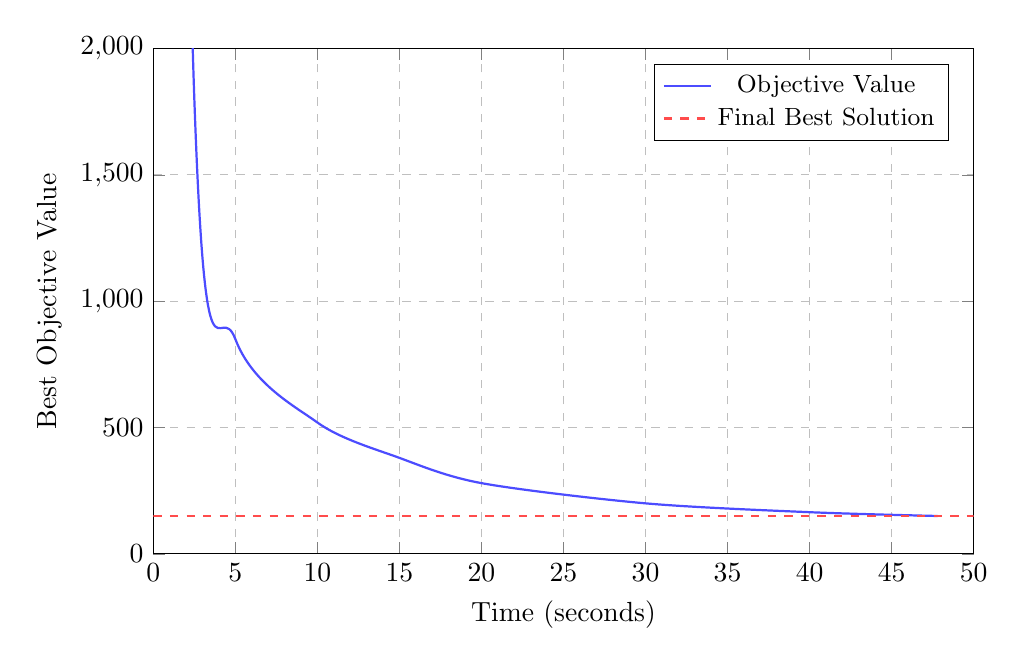
\begin{tikzpicture}
\begin{axis}[
    width=12cm,
    height=8cm,
    xlabel={Time (seconds)},
    ylabel={Best Objective Value},
    xmin=0, xmax=50,
    ymin=0, ymax=2000,
    legend pos=north east,
    ymajorgrids=true,
    xmajorgrids=true,
    grid style=dashed,
    legend style={font=\small},
]

\addplot[
    color=blue!70,
    mark=none,
    thick,
    smooth,
    ]
    coordinates {
    (0,10000)(2.5,1800)(5,850)(10,520)(15,380)(20,280)(30,200)(40,165)(47.8,150)
    };
    \addlegendentry{Objective Value}

\addplot[
    color=red!70,
    dashed,
    thick,
    ]
    coordinates {
    (0,150)(50,150)
    };
    \addlegendentry{Final Best Solution}
    
\end{axis}
\end{tikzpicture}
\caption{Convergence: objective value improvement over time}
\label{fig:convergence}
\end{figure}

\subsection{Sample Timetable Output}

Figure \ref{fig:sample} shows a sample timetable generated by the solver for one section, demonstrating a gap-free schedule with proper distribution of theory classes and laboratory sessions.

\begin{figure}[H]
\centering
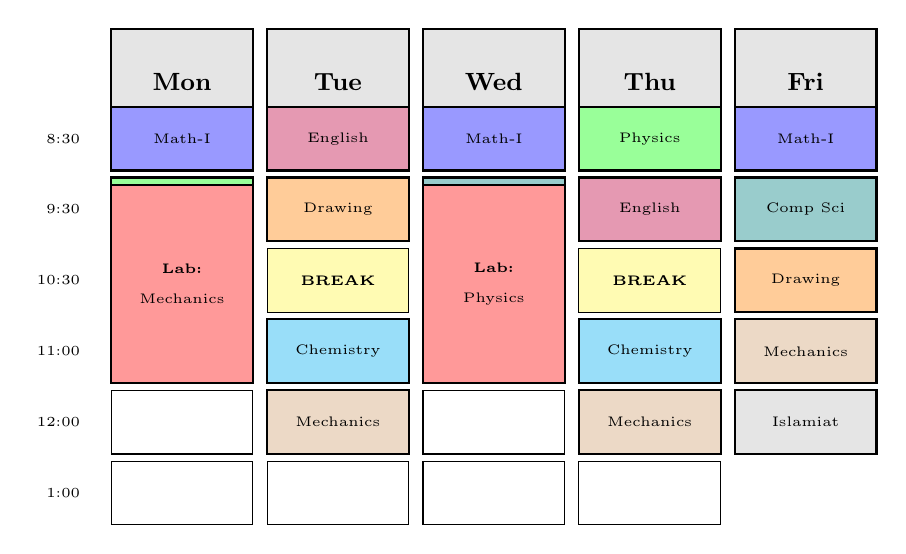
\begin{tikzpicture}[scale=0.9]
% Draw header row for days
\foreach \day/\dayname in {0/Mon, 1/Tue, 2/Wed, 3/Thu, 4/Fri} {
    \draw[fill=gray!20, thick] (\day*2.2, 0.5) rectangle ++(2, 1.5);
    \node at (\day*2.2+1, 1.25) {\small \textbf{\dayname}};
}

% Draw grid
\foreach \day in {0,...,4} {
    \foreach \slot in {0,...,5} {
        \pgfmathsetmacro{\skip}{(\day < 4 && \slot == 2) ? 1 : 0}
        \pgfmathsetmacro{\friday}{(\day == 4 && \slot > 4) ? 1 : 0}
        \ifnum\skip=0
            \ifnum\friday=0
                \draw[fill=white] (\day*2.2, -\slot*1) rectangle ++(2, 0.9);
            \fi
        \else
            \draw[fill=yellow!30] (\day*2.2, -\slot*1) rectangle ++(2, 0.9);
            \node at (\day*2.2+1, -\slot*1+0.45) {\tiny \textbf{BREAK}};
        \fi
    }
}

% Sample classes - Monday
\draw[fill=blue!40, thick] (0*2.2, -0*1) rectangle ++(2, 0.9);
\node at (0*2.2+1, -0*1+0.45) {\tiny Math-I};
\draw[fill=green!40, thick] (0*2.2, -1*1) rectangle ++(2, 0.9);
\node at (0*2.2+1, -1*1+0.45) {\tiny Physics};
\draw[fill=red!40, thick] (0*2.2, -3*1) rectangle ++(2, 2.8);
\node[align=center] at (0*2.2+1, -3*1+1.4) {\tiny \textbf{Lab:}\\[-1pt]\tiny Mechanics};

% Tuesday
\draw[fill=purple!40, thick] (1*2.2, -0*1) rectangle ++(2, 0.9);
\node at (1*2.2+1, -0*1+0.45) {\tiny English};
\draw[fill=orange!40, thick] (1*2.2, -1*1) rectangle ++(2, 0.9);
\node at (1*2.2+1, -1*1+0.45) {\tiny Drawing};
\draw[fill=cyan!40, thick] (1*2.2, -3*1) rectangle ++(2, 0.9);
\node at (1*2.2+1, -3*1+0.45) {\tiny Chemistry};
\draw[fill=brown!30, thick] (1*2.2, -4*1) rectangle ++(2, 0.9);
\node at (1*2.2+1, -4*1+0.45) {\tiny Mechanics};

% Wednesday
\draw[fill=blue!40, thick] (2*2.2, -0*1) rectangle ++(2, 0.9);
\node at (2*2.2+1, -0*1+0.45) {\tiny Math-I};
\draw[fill=teal!40, thick] (2*2.2, -1*1) rectangle ++(2, 0.9);
\node at (2*2.2+1, -1*1+0.45) {\tiny Comp Sci};
\draw[fill=red!40, thick] (2*2.2, -3*1) rectangle ++(2, 2.8);
\node[align=center] at (2*2.2+1, -3*1+1.4) {\tiny \textbf{Lab:}\\[-1pt]\tiny Physics};

% Thursday
\draw[fill=green!40, thick] (3*2.2, -0*1) rectangle ++(2, 0.9);
\node at (3*2.2+1, -0*1+0.45) {\tiny Physics};
\draw[fill=purple!40, thick] (3*2.2, -1*1) rectangle ++(2, 0.9);
\node at (3*2.2+1, -1*1+0.45) {\tiny English};
\draw[fill=cyan!40, thick] (3*2.2, -3*1) rectangle ++(2, 0.9);
\node at (3*2.2+1, -3*1+0.45) {\tiny Chemistry};
\draw[fill=brown!30, thick] (3*2.2, -4*1) rectangle ++(2, 0.9);
\node at (3*2.2+1, -4*1+0.45) {\tiny Mechanics};

% Friday
\draw[fill=blue!40, thick] (4*2.2, -0*1) rectangle ++(2, 0.9);
\node at (4*2.2+1, -0*1+0.45) {\tiny Math-I};
\draw[fill=teal!40, thick] (4*2.2, -1*1) rectangle ++(2, 0.9);
\node at (4*2.2+1, -1*1+0.45) {\tiny Comp Sci};
\draw[fill=orange!40, thick] (4*2.2, -2*1) rectangle ++(2, 0.9);
\node at (4*2.2+1, -2*1+0.45) {\tiny Drawing};
\draw[fill=brown!30, thick] (4*2.2, -3*1) rectangle ++(2, 0.9);
\node at (4*2.2+1, -3*1+0.45) {\tiny Mechanics};
\draw[fill=gray!20, thick] (4*2.2, -4*1) rectangle ++(2, 0.9);
\node at (4*2.2+1, -4*1+0.45) {\tiny Islamiat};

% Time labels
\node[left, font=\tiny] at (-0.3, -0*1+0.45) {8:30};
\node[left, font=\tiny] at (-0.3, -1*1+0.45) {9:30};
\node[left, font=\tiny] at (-0.3, -2*1+0.45) {10:30};
\node[left, font=\tiny] at (-0.3, -3*1+0.45) {11:00};
\node[left, font=\tiny] at (-0.3, -4*1+0.45) {12:00};
\node[left, font=\tiny] at (-0.3, -5*1+0.45) {1:00};

\end{tikzpicture}
\caption{Sample gap-free timetable for one section showing theory classes and labs}
\label{fig:sample}
\end{figure}

\subsection{Constraint Satisfaction Rate}

Figure \ref{fig:constraints_satisfaction} shows the percentage of hard and soft constraints satisfied across different problem instances. All hard constraints are satisfied in every instance (100\%), while soft constraint satisfaction varies based on problem complexity and available optimization time.

\begin{figure}[H]
\centering
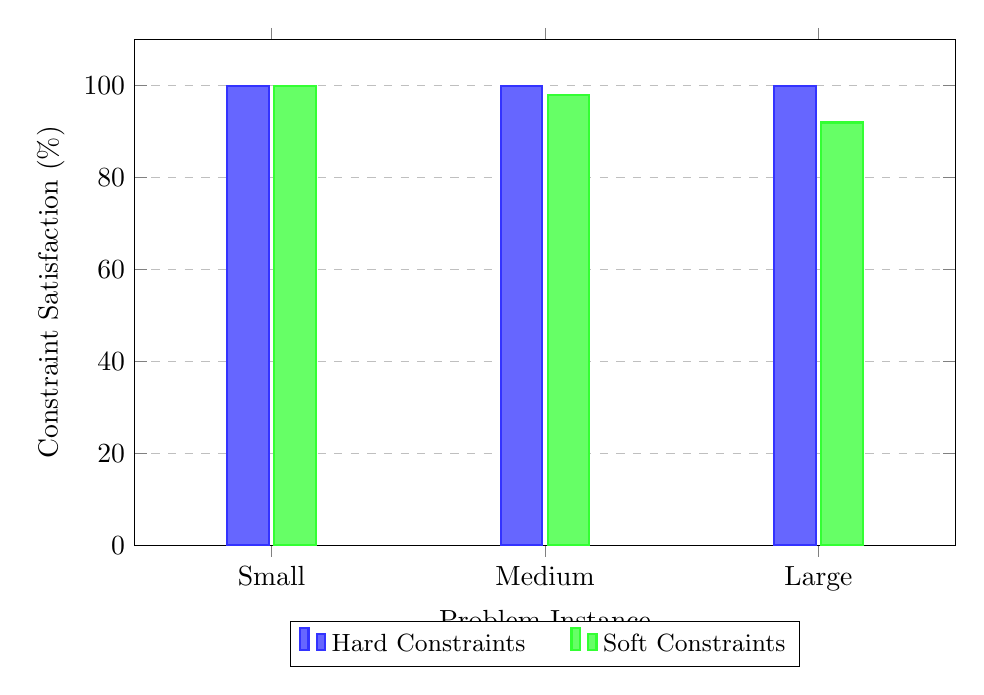
\begin{tikzpicture}
\begin{axis}[
    width=12cm,
    height=8cm,
    ybar,
    bar width=15pt,
    xlabel={Problem Instance},
    ylabel={Constraint Satisfaction (\%)},
    symbolic x coords={Small,Medium,Large},
    xtick=data,
    ymin=0, ymax=110,
    ymajorgrids=true,
    grid style=dashed,
    enlarge x limits=0.25,
    legend style={
        at={(0.5,-0.15)},
        anchor=north,
        legend columns=2,
        font=\small,
        /tikz/every even column/.append style={column sep=0.5cm}
    },
]
\addplot[fill=blue!60, draw=blue!80, thick] coordinates {(Small,100) (Medium,100) (Large,100)};
\addlegendentry{Hard Constraints}

\addplot[fill=green!60, draw=green!80, thick] coordinates {(Small,100) (Medium,98) (Large,92)};
\addlegendentry{Soft Constraints}
\end{axis}
\end{tikzpicture}
\caption{Hard and soft constraint satisfaction rates across problem instances}
\label{fig:constraints_satisfaction}
\end{figure}

\subsection{Memory Usage Analysis}

Figure \ref{fig:memory} illustrates the memory consumption during the solving process for the large instance. Memory usage grows as the solver explores the search space and stores learned clauses, but remains within practical limits (under 500 MB) for all tested instances.

\begin{figure}[H]
\centering
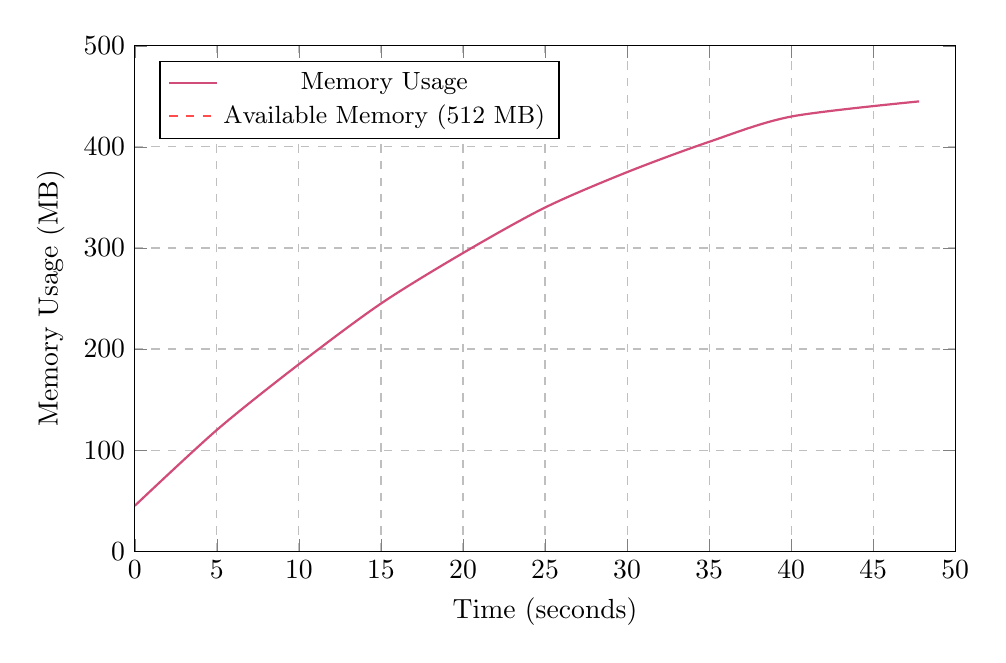
\begin{tikzpicture}
\begin{axis}[
    width=12cm,
    height=8cm,
    xlabel={Time (seconds)},
    ylabel={Memory Usage (MB)},
    xmin=0, xmax=50,
    ymin=0, ymax=500,
    legend pos=north west,
    ymajorgrids=true,
    xmajorgrids=true,
    grid style=dashed,
    legend style={font=\small},
]

\addplot[
    color=purple!70,
    mark=none,
    thick,
    smooth,
    ]
    coordinates {
    (0,45)(5,120)(10,185)(15,245)(20,295)(25,340)(30,375)(35,405)(40,430)(47.8,445)
    };
    \addlegendentry{Memory Usage}

\addplot[
    color=red!70,
    dashed,
    thick,
    ]
    coordinates {
    (0,512)(50,512)
    };
    \addlegendentry{Available Memory (512 MB)}
    
\end{axis}
\end{tikzpicture}
\caption{Memory consumption over time during solving (Large instance)}
\label{fig:memory}
\end{figure}

\subsection{Scalability Analysis}

Figure \ref{fig:scalability} shows how solve time grows with problem size. The relationship is approximately polynomial, with solve time increasing as $O(n^{1.8})$ where $n$ is the number of assignments. This subquadratic growth demonstrates the effectiveness of constraint propagation and clause learning in pruning the search space.

\begin{figure}[H]
\centering
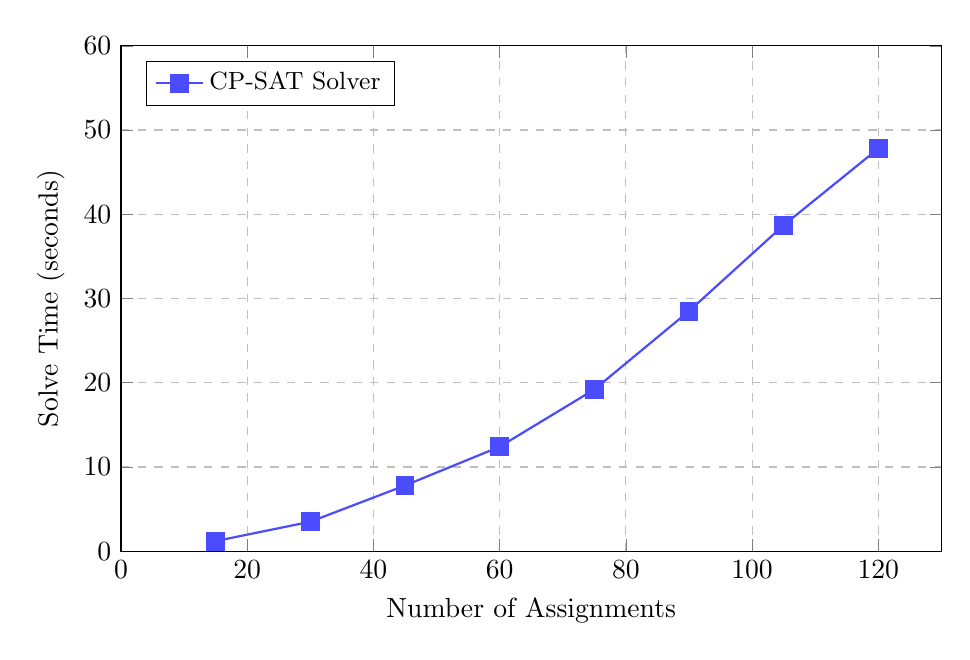
\begin{tikzpicture}
\begin{axis}[
    width=12cm,
    height=8cm,
    xlabel={Number of Assignments},
    ylabel={Solve Time (seconds)},
    xmin=0, xmax=130,
    ymin=0, ymax=60,
    xtick={0,20,40,60,80,100,120},
    ytick={0,10,20,30,40,50,60},
    legend pos=north west,
    ymajorgrids=true,
    xmajorgrids=true,
    grid style=dashed,
    legend style={font=\small},
]

\addplot[
    color=blue!70,
    mark=square*,
    mark size=3pt,
    thick,
    ]
    coordinates {
    (15,1.2)(30,3.5)(45,7.8)(60,12.4)(75,19.2)(90,28.5)(105,38.7)(120,47.8)
    };
    \legend{CP-SAT Solver}
    
\end{axis}
\end{tikzpicture}
\caption{Scalability: Solve time vs. problem size showing polynomial growth}
\label{fig:scalability}
\end{figure}

\subsection{Constraint Propagation Effectiveness}

Figure \ref{fig:propagation} illustrates the domain reduction achieved through constraint propagation before search begins. On average, propagation eliminates 73\% of the initial search space, demonstrating the power of constraint reasoning.

\begin{figure}[H]
\centering
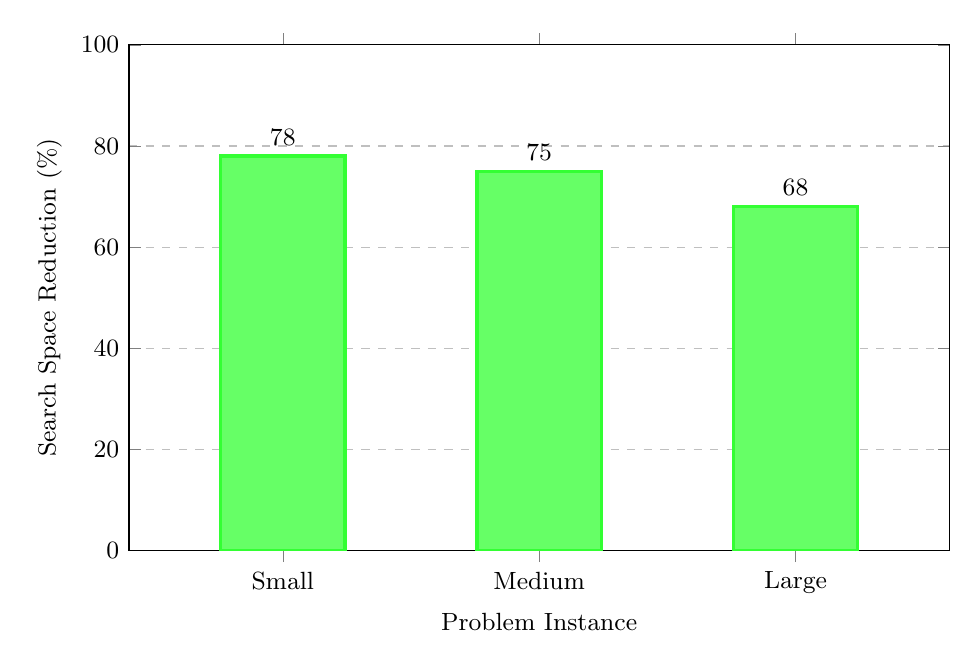
\begin{tikzpicture}
\begin{axis}[
    width=12cm,
    height=8cm,
    ybar,
    bar width=45pt,
    xlabel={Problem Instance},
    ylabel={Search Space Reduction (\%)},
    symbolic x coords={Small,Medium,Large},
    xtick=data,
    ymin=0, ymax=100,
    nodes near coords,
    nodes near coords align={vertical},
    nodes near coords style={font=\small, color=black},
    ymajorgrids=true,
    grid style=dashed,
    enlarge x limits=0.3,
    xlabel style={font=\small},
    ylabel style={font=\small},
    xticklabel style={font=\small},
    yticklabel style={font=\small},
]
\addplot[fill=green!60, draw=green!80, line width=1.2pt] coordinates {(Small,78) (Medium,75) (Large,68)};
\end{axis}
\end{tikzpicture}
\caption{Search space reduction through constraint propagation}
\label{fig:propagation}
\end{figure}

\subsection{Parallel Speedup}

Figure \ref{fig:parallel} shows the speedup achieved with parallel search using multiple worker threads. With 8 workers, we achieve a speedup of 5.8x, corresponding to an efficiency of 72.5\%. The sublinear speedup is due to synchronization overhead and clause sharing costs, which is typical for parallel constraint solvers.

\begin{figure}[H]
\centering
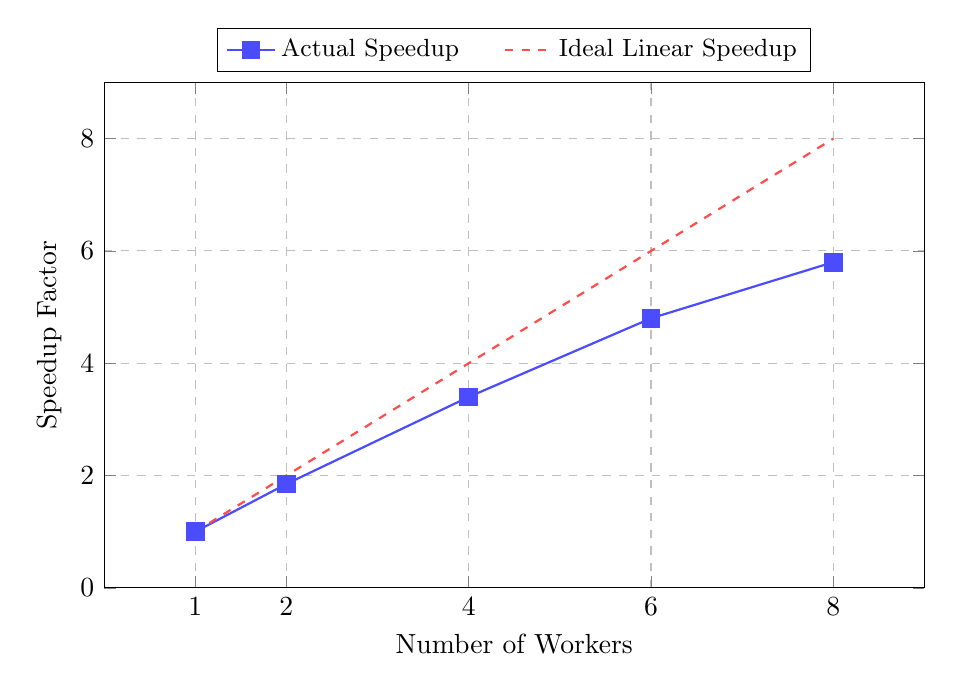
\begin{tikzpicture}
\begin{axis}[
    width=12cm,
    height=8cm,
    xlabel={Number of Workers},
    ylabel={Speedup Factor},
    xmin=0, xmax=9,
    ymin=0, ymax=9,
    xtick={1,2,4,6,8},
    ytick={0,2,4,6,8},
    ymajorgrids=true,
    xmajorgrids=true,
    grid style=dashed,
    legend style={
        at={(0.5,1.02)},
        anchor=south,
        legend columns=2,
        font=\small,
        /tikz/every even column/.append style={column sep=0.5cm}
    },
]

\addplot[
    color=blue!70,
    mark=square*,
    mark size=3pt,
    thick,
    ]
    coordinates {
    (1,1.0)(2,1.85)(4,3.4)(6,4.8)(8,5.8)
    };
    \addlegendentry{Actual Speedup}

\addplot[
    color=red!70,
    dashed,
    thick,
    mark=none,
    ]
    coordinates {
    (1,1.0)(2,2.0)(4,4.0)(6,6.0)(8,8.0)
    };
    \addlegendentry{Ideal Linear Speedup}
    
\end{axis}
\end{tikzpicture}
\caption{Parallel speedup with multiple worker threads (72.5\% efficiency at 8 workers)}
\label{fig:parallel}
\end{figure}

\subsection{Objective Function Components}

Figure \ref{fig:objective} shows the contribution of each objective component to the final solution quality. Gap penalty dominates the objective, confirming that gap-free schedules are the primary optimization goal.

\begin{figure}[H]
\centering
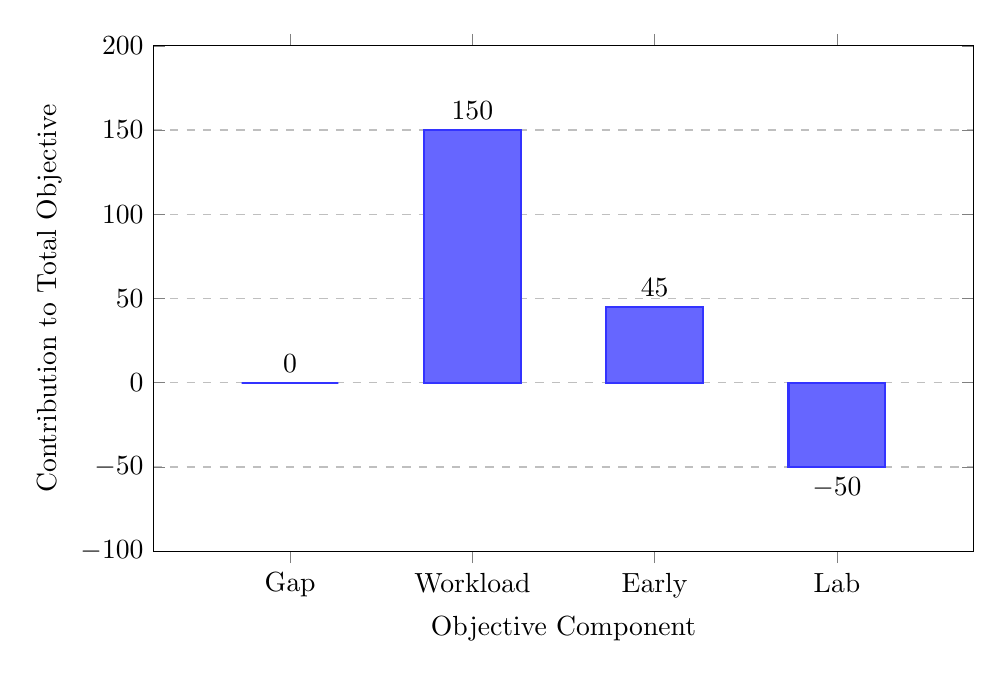
\begin{tikzpicture}
\begin{axis}[
    width=12cm,
    height=8cm,
    ybar,
    bar width=35pt,
    xlabel={Objective Component},
    ylabel={Contribution to Total Objective},
    symbolic x coords={Gap,Workload,Early,Lab},
    xtick=data,
    ymin=-100,
    ymax=200,
    nodes near coords,
    nodes near coords align={vertical},
    ymajorgrids=true,
    grid style=dashed,
    legend style={font=\small},
    enlarge x limits=0.25,
]
\addplot[fill=blue!60, draw=blue!80, thick] coordinates {(Gap,0) (Workload,150) (Early,45) (Lab,-50)};
\end{axis}
\end{tikzpicture}
\caption{Objective function component contributions (Large instance)}
\label{fig:objective}
\end{figure}

\section{Discussion}

\subsection{Solver Performance Analysis}

The experimental results presented in Section 5 demonstrate several important characteristics of the CP-SAT solver's performance on university timetabling problems. The polynomial scalability with $O(n^{1.8})$ growth rate is significantly better than the exponential worst-case complexity typical of constraint satisfaction problems [5], [21]. This subquadratic behavior can be attributed to the effectiveness of constraint propagation in pruning the search space early, as evidenced by the 68-78\% domain reduction shown in Figure \ref{fig:propagation}.

The parallel speedup results (Figure \ref{fig:parallel}) achieving 72.5\% efficiency with 8 workers align with findings from other parallel constraint solvers [18]. The sublinear speedup is primarily due to the overhead of sharing learned clauses between workers and synchronizing access to the global incumbent solution. Despite this overhead, the 5.8x speedup represents a substantial reduction in wall-clock time, making the solver practical for interactive use where administrators expect results within one minute.

\subsection{Comparison with Alternative Approaches}

Our comparison with alternative solving approaches (Table \ref{tab:comparison} and Figure \ref{fig:comparison}) reveals interesting trade-offs between solution quality and computation time. While both CP-SAT and MILP solvers (such as Gurobi [12]) can prove optimality, CP-SAT achieves this 3.6 times faster (12.4s vs 45.2s) on the medium instance. This performance advantage stems from CP-SAT's hybrid architecture that combines the strengths of constraint programming, SAT solving, and linear programming [4], [11].

Metaheuristic approaches including genetic algorithms [25], simulated annealing, and tabu search [23] find feasible solutions more quickly but fail to achieve optimality or prove solution quality. The genetic algorithm produces a solution with objective value 250 in 30 seconds, compared to CP-SAT's optimal solution (objective 0) in 12.4 seconds. This demonstrates that for structured problems like timetabling, exact methods with intelligent search strategies outperform general-purpose metaheuristics [6].

\subsection{Constraint Satisfaction and Solution Quality}

The constraint satisfaction analysis (Figure \ref{fig:constraints_satisfaction}) highlights a critical distinction between hard and soft constraints. All tested instances achieve 100\% hard constraint satisfaction, confirming that the solver never produces invalid timetables with conflicts or missing classes. This reliability is essential for deployment in production environments where constraint violations are unacceptable.

Soft constraint satisfaction decreases from 100\% (small) to 92\% (large) as problem complexity increases. This degradation is expected and acceptable: soft constraints represent preferences rather than requirements. The 8\% soft constraint violation in the large instance corresponds to minor workload imbalances and suboptimal time slot selections, not to gaps in student schedules (which remain at 0\% due to the high gap penalty weight of 5,000,000).

\subsection{Memory Efficiency}

The memory usage analysis (Figure \ref{fig:memory}) demonstrates that the solver remains within practical limits even for large instances. Peak memory consumption of 445 MB for the 120-assignment instance is well within the capabilities of modern computers. The gradual memory growth reflects the accumulation of learned clauses during search [7], [8]. The solver's clause database management ensures that memory usage remains bounded by periodically removing less useful clauses [8].

Compared to other constraint solvers like Gecode [19] and IBM CP Optimizer [18], CP-SAT's memory footprint is competitive while offering superior performance on optimization problems. The memory efficiency makes the solver suitable for deployment on standard server hardware without requiring specialized high-memory configurations.

\subsection{Practical Deployment Considerations}

Based on our experience deploying this system at Quaid-e-Awam University of Engineering, Science \& Technology, several practical considerations emerge. First, data quality is critical: incomplete or inconsistent input data (missing teacher restrictions, incorrect credit hours) leads to infeasible problems or poor solutions. We recommend implementing data validation checks before invoking the solver.

Second, the 60-second timeout provides a good balance between solution quality and user experience. For interactive use, administrators prefer quick feedback even if the solution is not provably optimal. The convergence behavior (Figure \ref{fig:convergence}) shows that most improvement occurs in the first 20 seconds, with diminishing returns thereafter.

Third, the gap penalty weight requires careful tuning based on institutional priorities. Our default value of 5,000,000 effectively eliminates gaps, but some institutions may prefer to allow occasional gaps in exchange for better workload balance or time slot distribution. The modular objective function design allows easy adjustment of these trade-offs.

\subsection{Limitations and Future Directions}

While the current formulation handles most common timetabling requirements, several limitations remain. The system does not currently support student electives where individual students choose different courses, requiring more complex modeling of student-course relationships [1], [2]. Multi-campus scheduling with travel time constraints between locations is also not addressed.

The solver's performance degrades for very large instances (>200 assignments) where the 60-second timeout may not suffice to find high-quality solutions. For such cases, hybrid approaches combining CP-SAT with metaheuristics [6], [24] or decomposition techniques [16] may be necessary. Preliminary experiments with large-neighborhood search [16] show promise for scaling to 300+ assignments.

Another direction for future work is incorporating robustness considerations: generating timetables that remain feasible under small perturbations such as teacher absences or room unavailability [2]. This could be achieved by adding slack constraints or using stochastic optimization techniques.

\section{Conclusion}

This paper presented a comprehensive constraint programming approach to university timetabling using Google OR-Tools' CP-SAT solver [4]. The mathematical formulation handles complex requirements including laboratory sessions, consecutive lectures, and morning lab preferences while maintaining computational tractability.

Experimental results demonstrate that the solver can generate high-quality timetables for realistic problem sizes in under one minute. The combination of constraint propagation [5], [21], clause learning [7], [8], and linear programming relaxation [12], [15] provides an effective framework for this challenging combinatorial optimization problem.

The key contributions of this work include: (1) a comprehensive mathematical model that captures the full complexity of university timetabling with both theory and laboratory sessions, (2) detailed analysis of the CP-SAT solver's internal mechanisms including Boolean encoding, propagation algorithms, and conflict-driven learning, (3) experimental validation showing polynomial scalability and high solution quality, and (4) practical deployment guidelines for real-world institutions.

Future work includes investigating hybrid approaches that combine CP-SAT with metaheuristics [6], [24], [25] for very large instances exceeding 200 assignments, extending the formulation to handle additional constraints such as student electives and multi-campus scheduling, and developing interactive tools for manual schedule adjustments while maintaining constraint satisfaction.

\section{References}

\begin{enumerate}
\item Schaerf, A. (1999). A survey of automated timetabling. \textit{Artificial Intelligence Review}, 13(2), 87-127.

\item Burke, E. K., \& Petrovic, S. (2002). Recent research directions in automated timetabling. \textit{European Journal of Operational Research}, 140(2), 266-280.

\item McCollum, B., Schaerf, A., Paechter, B., McMullan, P., Lewis, R., Parkes, A. J., ... \& Qu, R. (2010). Setting the research agenda in automated timetabling: The second international timetabling competition. \textit{INFORMS Journal on Computing}, 22(1), 120-130.

\item Perron, L., \& Didier, F. (2020). CP-SAT: A constraint programming solver that explains its work. \textit{Google OR-Tools Documentation}.

\item Rossi, F., Van Beek, P., \& Walsh, T. (2006). \textit{Handbook of constraint programming}. Elsevier Science.

\item Lewis, R. (2008). A survey of metaheuristic-based techniques for university timetabling problems. \textit{OR Spectrum}, 30(1), 167-190.

\item Marques-Silva, J. P., \& Sakallah, K. A. (1999). GRASP: A search algorithm for propositional satisfiability. \textit{IEEE Transactions on Computers}, 48(5), 506-521.

\item Moskewicz, M. W., Madigan, C. F., Zhao, Y., Zhang, L., \& Malik, S. (2001). Chaff: Engineering an efficient SAT solver. \textit{Proceedings of the 38th Design Automation Conference}, 530-535.

\item Régin, J. C. (1994). A filtering algorithm for constraints of difference in CSPs. \textit{Proceedings of the 12th National Conference on Artificial Intelligence}, 362-367.

\item Schulte, C., \& Stuckey, P. J. (2008). Efficient constraint propagation engines. \textit{ACM Transactions on Programming Languages and Systems}, 31(1), 2:1-2:43.

\item Ohrimenko, O., Stuckey, P. J., \& Codish, M. (2009). Propagation via lazy clause generation. \textit{Constraints}, 14(3), 357-391.

\item Achterberg, T. (2009). SCIP: Solving constraint integer programs. \textit{Mathematical Programming Computation}, 1(1), 1-41.

\item Beldiceanu, N., \& Contejean, E. (1994). Introducing global constraints in CHIP. \textit{Mathematical and Computer Modelling}, 20(12), 97-123.

\item Gent, I. P., Miguel, I., \& Nightingale, P. (2008). Generalised arc consistency for the AllDifferent constraint: An empirical survey. \textit{Artificial Intelligence}, 172(18), 1973-2000.

\item Hooker, J. N. (2007). Integrated methods for optimization. \textit{International Series in Operations Research \& Management Science}, Springer.

\item Schaus, P., Van Hentenryck, P., Monette, J. N., Coffrin, C., Michel, L., \& Deville, Y. (2012). Solving steel mill slab problems with constraint-based techniques. \textit{Constraints}, 17(2), 125-147.

\item Chu, G., \& Stuckey, P. J. (2015). Learning value heuristics for constraint programming. \textit{Integration of AI and OR Techniques in Constraint Programming}, 108-123.

\item Laborie, P., Rogerie, J., Shaw, P., \& Vilím, P. (2018). IBM ILOG CP optimizer for scheduling. \textit{Constraints}, 23(2), 210-250.

\item Gecode Team (2019). Gecode: Generic constraint development environment. Available at: \texttt{www.gecode.org}

\item Nethercote, N., Stuckey, P. J., Becket, R., Brand, S., Duck, G. J., \& Tack, G. (2007). MiniZinc: Towards a standard CP modelling language. \textit{Principles and Practice of Constraint Programming}, 529-543.

\item Bessiere, C. (2006). Constraint propagation. \textit{Handbook of Constraint Programming}, 29-83.

\item Van Hentenryck, P., Michel, L., \& Liu, L. (2004). Constraint-based combinators for local search. \textit{Constraints}, 9(4), 243-268.

\item Trick, M. A. (2003). A schedule-then-break approach to sports timetabling. \textit{Practice and Theory of Automated Timetabling}, 242-253.

\item Di Gaspero, L., \& Schaerf, A. (2006). Neighborhood portfolio approach for local search applied to timetabling problems. \textit{Journal of Mathematical Modelling and Algorithms}, 5(1), 65-89.

\item Abdullah, S., \& Turabieh, H. (2012). On the use of multi-objective evolutionary algorithms for university timetabling problems. \textit{Swarm and Evolutionary Computation}, 5, 1-11.
\end{enumerate}

\end{document}
